% !TeX encoding = UTF-8
% !TeX program = xelatex
% !TeX spellcheck = en_US

\documentclass[degree=bachelor,fontset=windows]{thuthesis}
  % 学位 degree:
  %   doctor | master | bachelor | postdoc
  % 学位类型 degree-type:
  %   academic(默认)| professional


% 论文基本配置,加载宏包等全局配置
% !TeX root = ../main.tex

% 论文基本信息配置

\thusetup{
  %******************************
  % 注意:
  %   1. 配置里面不要出现空行
  %   2. 不需要的配置信息可以删除
  %******************************
  %
  % 标题
  %   可使用“\\”命令手动控制换行
  %
  title  = {面向文档级关系抽取的预训练模型研究},
  title* = {Pre-training for Document-level Distantly Supervised Relation Extraction},
  %
  % 学位
  %   1. 学术型
  %      - 中文
  %        需注明所属的学科门类,例如:
  %        哲学、经济学、法学、教育学、文学、历史学、理学、工学、农学、医学、
  %        军事学、管理学、艺术学
  %      - 英文
  %        博士:Doctor of Philosophy
  %        硕士:
  %          哲学、文学、历史学、法学、教育学、艺术学门类,公共管理学科
  %          填写“Master of Arts“,其它填写“Master of Science”
  %   2. 专业型
  %      直接填写专业学位的名称,例如:
  %      教育博士、工程硕士等
  %      Doctor of Education, Master of Engineering
  %   3. 本科生不需要填写
  %
  degree-name  = {工学学士},
  degree-name* = {Master of Science},
  %
  % 培养单位
  %   填写所属院系的全名
  %
  department = {计算机科学与技术系},
  %
  % 学科
  %   1. 学术型学位
  %      获得一级学科授权的学科填写一级学科名称,其他填写二级学科名称
  %   2. 工程硕士
  %      工程领域名称
  %   3. 其他专业型学位
  %      不填写此项
  %   4. 本科生不需要填写
  %
  discipline  = {计算机科学与技术},
  discipline* = {Computer Science and Technology},
  %
  % 姓名
  %
  author  = {肖朝军},
  author* = {Xiao Chaojun},
  %
  % 指导教师
  %   中文姓名和职称之间以英文逗号“,”分开,下同
  %
  supervisor  = {刘知远副教授},
  supervisor* = {Associate Professor Liu Zhiyuan},
  %
  % 副指导教师
  %
  %associate-supervisor  = {陈文光教授},
  %associate-supervisor* = {Professor Chen Wenguang},
  %
  % 联合指导教师
  %
  % joint-supervisor  = {某某某教授},
  % joint-supervisor* = {Professor Mou Moumou},
  %
  % 日期
  %   使用 ISO 格式;默认为当前时间
  %
  % date = {2019-07-07},
  %
  % 密级和年限
  %   秘密, 机密, 绝密
  %
  % secret-level = {秘密},
  % secret-year  = {10},
  %
  % 博士后专有部分
  %
  % clc                = {分类号},
  % udc                = {UDC},
  % id                 = {编号},
  % discipline-level-1 = {计算机科学与技术},  % 流动站(一级学科)名称
  % discipline-level-2 = {系统结构},          % 专业(二级学科)名称
  % start-date         = {2011-07-01},        % 研究工作起始时间
}

%% Put any packages you would like to use here

% 表格中支持跨行
\usepackage{multirow}

% 跨页表格
\usepackage{longtable}

% 固定宽度的表格
\usepackage{tabularx}

% 表格中的反斜线
\usepackage{diagbox}

% 确定浮动对象的位置,可以使用 H,强制将浮动对象放到这里(可能效果很差)
\usepackage{float}

% 浮动图形控制宏包。
% 允许上一个 section 的浮动图形出现在下一个 section 的开始部分
% 该宏包提供处理浮动对象的 \FloatBarrier 命令,使所有未处
% 理的浮动图形立即被处理。这三个宏包仅供参考,未必使用:
% \usepackage[below]{placeins}
% \usepackage{floatflt} % 图文混排用宏包
% \usepackage{rotating} % 图形和表格的控制旋转

% 定理类环境宏包
\usepackage[amsmath,thmmarks,hyperref]{ntheorem}

% 给自定义的宏后面自动加空白
% \usepackage{xspace}

% 借用 ltxdoc 里面的几个命令。
\def\cmd#1{\cs{\expandafter\cmd@to@cs\string#1}}
\def\cmd@to@cs#1#2{\char\number`#2\relax}
\DeclareRobustCommand\cs[1]{\texttt{\char`\\#1}}

\newcommand*{\meta}[1]{{%
  \ensuremath{\langle}\rmfamily\itshape#1\/\ensuremath{\rangle}}}
\providecommand\marg[1]{%
  {\ttfamily\char`\{}\meta{#1}{\ttfamily\char`\}}}
\providecommand\oarg[1]{%
  {\ttfamily[}\meta{#1}{\ttfamily]}}
\providecommand\parg[1]{%
  {\ttfamily(}\meta{#1}{\ttfamily)}}
\providecommand\pkg[1]{{\sffamily#1}}

% 定义所有的图片文件在 figures 子目录下
\graphicspath{{figures/}}

% 数学命令
% Adapted for use with thuthesis.
% Original code is at https://github.com/goodfeli/dlbook_notation/blob/master/math_commands.tex

%%%%% NEW MATH DEFINITIONS %%%%%

\newcommand\ceil[1]{\lceil #1 \rceil}
\newcommand\floor[1]{\lfloor #1 \rfloor}


% Vectors
\newcommand\Vector[1]{\symbf{#1}}

\newcommand\0{{\Vector{0}}}
\newcommand\vzero{{\Vector{0}}}
\newcommand\1{{\Vector{1}}}
\newcommand\vone{{\Vector{1}}}

\newcommand\va{{\Vector{a}}}
\newcommand\vb{{\Vector{b}}}
\newcommand\vc{{\Vector{c}}}
\newcommand\vd{{\Vector{d}}}
\newcommand\ve{{\Vector{e}}}
\newcommand\vf{{\Vector{f}}}
\newcommand\vg{{\Vector{g}}}
\newcommand\vh{{\Vector{h}}}
\newcommand\vi{{\Vector{i}}}
\newcommand\vj{{\Vector{j}}}
\newcommand\vk{{\Vector{k}}}
\newcommand\vl{{\Vector{l}}}
\newcommand\vm{{\Vector{m}}}
\newcommand\vn{{\Vector{n}}}
\newcommand\vo{{\Vector{o}}}
\newcommand\vp{{\Vector{p}}}
\newcommand\vq{{\Vector{q}}}
\newcommand\vr{{\Vector{r}}}
\newcommand\vs{{\Vector{s}}}
\newcommand\vt{{\Vector{t}}}
\newcommand\vu{{\Vector{u}}}
\newcommand\vv{{\Vector{v}}}
\newcommand\vw{{\Vector{w}}}
\newcommand\vx{{\Vector{x}}}
\newcommand\vy{{\Vector{y}}}
\newcommand\vz{{\Vector{z}}}

\newcommand\valpha{{\Vector{\alpha}}}
\newcommand\vbeta{{\Vector{\beta}}}
\newcommand\vgamma{{\Vector{\gamma}}}
\newcommand\vdelta{{\Vector{\delta}}}
\newcommand\vepsilon{{\Vector{\epsilon}}}
\newcommand\vtheta{{\Vector{\theta}}}
\newcommand\viota{{\Vector{\iota}}}
\newcommand\vkappa{{\Vector{\kappa}}}
\newcommand\vlambda{{\Vector{\lambda}}}
\newcommand\vmu{{\Vector{\mu}}}
\newcommand\vnu{{\Vector{\nu}}}
\newcommand\vxi{{\Vector{\xi}}}
\newcommand\vpi{{\Vector{\pi}}}
\newcommand\vrho{{\Vector{\rho}}}
\newcommand\vsigma{{\Vector{\sigma}}}
\newcommand\vtau{{\Vector{\tau}}}
\newcommand\vupsilon{{\Vector{\upsilon}}}
\newcommand\vphi{{\Vector{\phi}}}
\newcommand\vchi{{\Vector{\chi}}}
\newcommand\vpsi{{\Vector{\psi}}}
\newcommand\vomega{{\Vector{\omega}}}


% Matrix
\newcommand\MATRIX[1]{\symbf{#1}}

\newcommand\mA{{\MATRIX{A}}}
\newcommand\mB{{\MATRIX{B}}}
\newcommand\mC{{\MATRIX{C}}}
\newcommand\mD{{\MATRIX{D}}}
\newcommand\mE{{\MATRIX{E}}}
\newcommand\mF{{\MATRIX{F}}}
\newcommand\mG{{\MATRIX{G}}}
\newcommand\mH{{\MATRIX{H}}}
\newcommand\mI{{\MATRIX{I}}}
\newcommand\mJ{{\MATRIX{J}}}
\newcommand\mK{{\MATRIX{K}}}
\newcommand\mL{{\MATRIX{L}}}
\newcommand\mM{{\MATRIX{M}}}
\newcommand\mN{{\MATRIX{N}}}
\newcommand\mO{{\MATRIX{O}}}
\newcommand\mP{{\MATRIX{P}}}
\newcommand\mQ{{\MATRIX{Q}}}
\newcommand\mR{{\MATRIX{R}}}
\newcommand\mS{{\MATRIX{S}}}
\newcommand\mT{{\MATRIX{T}}}
\newcommand\mU{{\MATRIX{U}}}
\newcommand\mV{{\MATRIX{V}}}
\newcommand\mW{{\MATRIX{W}}}
\newcommand\mX{{\MATRIX{X}}}
\newcommand\mY{{\MATRIX{Y}}}
\newcommand\mZ{{\MATRIX{Z}}}

\newcommand\mGamma{{\MATRIX{\Gamma}}}
\newcommand\mDelta{{\MATRIX{\Delta}}}
\newcommand\mTheta{{\MATRIX{\Theta}}}
\newcommand\mLambda{{\MATRIX{\Lambda}}}
\newcommand\mXi{{\MATRIX{\Xi}}}
\newcommand\mPi{{\MATRIX{\Pi}}}
\newcommand\mSigma{{\MATRIX{\Sigma}}}
\newcommand\mUpsilon{{\MATRIX{\Upsilon}}}
\newcommand\mPhi{{\MATRIX{\Phi}}}
\newcommand\mPsi{{\MATRIX{\Psi}}}
\newcommand\mOmega{{\MATRIX{\Omega}}}


% Tensor
\newcommand\tens[1]{\symbfsf{#1}}
\newcommand\tA{{\tens{A}}}
\newcommand\tB{{\tens{B}}}
\newcommand\tC{{\tens{C}}}
\newcommand\tD{{\tens{D}}}
\newcommand\tE{{\tens{E}}}
\newcommand\tF{{\tens{F}}}
\newcommand\tG{{\tens{G}}}
\newcommand\tH{{\tens{H}}}
\newcommand\tI{{\tens{I}}}
\newcommand\tJ{{\tens{J}}}
\newcommand\tK{{\tens{K}}}
\newcommand\tL{{\tens{L}}}
\newcommand\tM{{\tens{M}}}
\newcommand\tN{{\tens{N}}}
\newcommand\tO{{\tens{O}}}
\newcommand\tP{{\tens{P}}}
\newcommand\tQ{{\tens{Q}}}
\newcommand\tR{{\tens{R}}}
\newcommand\tS{{\tens{S}}}
\newcommand\tT{{\tens{T}}}
\newcommand\tU{{\tens{U}}}
\newcommand\tV{{\tens{V}}}
\newcommand\tW{{\tens{W}}}
\newcommand\tX{{\tens{X}}}
\newcommand\tY{{\tens{Y}}}
\newcommand\tZ{{\tens{Z}}}


% Graph
\newcommand\gA{{\mathcal{A}}}
\newcommand\gB{{\mathcal{B}}}
\newcommand\gC{{\mathcal{C}}}
\newcommand\gD{{\mathcal{D}}}
\newcommand\gE{{\mathcal{E}}}
\newcommand\gF{{\mathcal{F}}}
\newcommand\gG{{\mathcal{G}}}
\newcommand\gH{{\mathcal{H}}}
\newcommand\gI{{\mathcal{I}}}
\newcommand\gJ{{\mathcal{J}}}
\newcommand\gK{{\mathcal{K}}}
\newcommand\gL{{\mathcal{L}}}
\newcommand\gM{{\mathcal{M}}}
\newcommand\gN{{\mathcal{N}}}
\newcommand\gO{{\mathcal{O}}}
\newcommand\gP{{\mathcal{P}}}
\newcommand\gQ{{\mathcal{Q}}}
\newcommand\gR{{\mathcal{R}}}
\newcommand\gS{{\mathcal{S}}}
\newcommand\gT{{\mathcal{T}}}
\newcommand\gU{{\mathcal{U}}}
\newcommand\gV{{\mathcal{V}}}
\newcommand\gW{{\mathcal{W}}}
\newcommand\gX{{\mathcal{X}}}
\newcommand\gY{{\mathcal{Y}}}
\newcommand\gZ{{\mathcal{Z}}}


% Sets
\newcommand\sA{{\mathbb{A}}}
\newcommand\sB{{\mathbb{B}}}
\newcommand\sC{{\mathbb{C}}}
\newcommand\sD{{\mathbb{D}}}
% Don't use a set called E, because this would be the same as our symbol
% for expectation.
\newcommand\sF{{\mathbb{F}}}
\newcommand\sG{{\mathbb{G}}}
\newcommand\sH{{\mathbb{H}}}
\newcommand\sI{{\mathbb{I}}}
\newcommand\sJ{{\mathbb{J}}}
\newcommand\sK{{\mathbb{K}}}
\newcommand\sL{{\mathbb{L}}}
\newcommand\sM{{\mathbb{M}}}
\newcommand\sN{{\mathbb{N}}}
\newcommand\sO{{\mathbb{O}}}
\newcommand\sP{{\mathbb{P}}}
\newcommand\sQ{{\mathbb{Q}}}
\newcommand\sR{{\mathbb{R}}}
\newcommand\sS{{\mathbb{S}}}
\newcommand\sT{{\mathbb{T}}}
\newcommand\sU{{\mathbb{U}}}
\newcommand\sV{{\mathbb{V}}}
\newcommand\sW{{\mathbb{W}}}
\newcommand\sX{{\mathbb{X}}}
\newcommand\sY{{\mathbb{Y}}}
\newcommand\sZ{{\mathbb{Z}}}


% Random variables
\newcommand\RandomVariable[1]{\symit{#1}}

\newcommand\rA{{\RandomVariable{A}}}
\newcommand\rB{{\RandomVariable{B}}}
\newcommand\rC{{\RandomVariable{C}}}
\newcommand\rD{{\RandomVariable{D}}}
\newcommand\rE{{\RandomVariable{E}}}
\newcommand\rF{{\RandomVariable{F}}}
\newcommand\rG{{\RandomVariable{G}}}
\newcommand\rH{{\RandomVariable{H}}}
\newcommand\rI{{\RandomVariable{I}}}
\newcommand\rJ{{\RandomVariable{J}}}
\newcommand\rK{{\RandomVariable{K}}}
\newcommand\rL{{\RandomVariable{L}}}
\newcommand\rM{{\RandomVariable{M}}}
\newcommand\rN{{\RandomVariable{N}}}
\newcommand\rO{{\RandomVariable{O}}}
\newcommand\rP{{\RandomVariable{P}}}
\newcommand\rQ{{\RandomVariable{Q}}}
\newcommand\rR{{\RandomVariable{R}}}
\newcommand\rS{{\RandomVariable{S}}}
\newcommand\rT{{\RandomVariable{T}}}
\newcommand\rU{{\RandomVariable{U}}}
\newcommand\rV{{\RandomVariable{V}}}
\newcommand\rW{{\RandomVariable{W}}}
\newcommand\rX{{\RandomVariable{X}}}
\newcommand\rY{{\RandomVariable{Y}}}
\newcommand\rZ{{\RandomVariable{Z}}}

% Random vectors
\newcommand\RandomVector[1]{\symbf{#1}}

\newcommand\rvA{{\RandomVector{A}}}
\newcommand\rvB{{\RandomVector{B}}}
\newcommand\rvC{{\RandomVector{C}}}
\newcommand\rvD{{\RandomVector{D}}}
\newcommand\rvE{{\RandomVector{E}}}
\newcommand\rvF{{\RandomVector{F}}}
\newcommand\rvG{{\RandomVector{G}}}
\newcommand\rvH{{\RandomVector{H}}}
\newcommand\rvI{{\RandomVector{I}}}
\newcommand\rvJ{{\RandomVector{J}}}
\newcommand\rvK{{\RandomVector{K}}}
\newcommand\rvL{{\RandomVector{L}}}
\newcommand\rvM{{\RandomVector{M}}}
\newcommand\rvN{{\RandomVector{N}}}
\newcommand\rvO{{\RandomVector{O}}}
\newcommand\rvP{{\RandomVector{P}}}
\newcommand\rvQ{{\RandomVector{Q}}}
\newcommand\rvR{{\RandomVector{R}}}
\newcommand\rvS{{\RandomVector{S}}}
\newcommand\rvT{{\RandomVector{T}}}
\newcommand\rvU{{\RandomVector{U}}}
\newcommand\rvV{{\RandomVector{V}}}
\newcommand\rvW{{\RandomVector{W}}}
\newcommand\rvX{{\RandomVector{X}}}
\newcommand\rvY{{\RandomVector{Y}}}
\newcommand\rvZ{{\RandomVector{Z}}}

\newcommand\laplace{\mathrm{Laplace}} % Laplace distribution

\newcommand\E{\mathbb{E}}
\newcommand\Ls{\mathcal{L}}
\newcommand\R{\mathbb{R}}
\newcommand\emp{\tilde{p}}
\newcommand\lr{\alpha}
\newcommand\reg{\lambda}
\newcommand\rect{\mathrm{rectifier}}
\newcommand\softmax{\mathrm{softmax}}
\newcommand\sigmoid{\sigma}
\newcommand\softplus{\zeta}
\newcommand\KL{D_{\mathrm{KL}}}
\newcommand\Var{\mathrm{Var}}
\newcommand\standarderror{\mathrm{SE}}
\newcommand\Cov{\mathrm{Cov}}
% Wolfram Mathworld says $L^2$ is for function spaces and $\ell^2$ is for vectors
% But then they seem to use $L^2$ for vectors throughout the site, and so does
% wikipedia.
\newcommand\normlzero{L^0}
\newcommand\normlone{L^1}
\newcommand\normltwo{L^2}
\newcommand\normlp{L^p}
\newcommand\normmax{L^\infty}

\DeclareMathOperator*{\argmax}{arg\,max}
\DeclareMathOperator*{\argmin}{arg\,min}

\DeclareMathOperator{\sign}{sign}
\DeclareMathOperator{\Tr}{Tr}
\let\ab\allowbreak


% 定义自己常用的东西
% \def\myname{薛瑞尼}

% hyperref 宏包在最后调用
\usepackage{hyperref}



\begin{document}

% 封面
\maketitle

% 使用授权的说明
\copyrightpage

\frontmatter
% !TeX root = ../main.tex

% 中英文摘要和关键字

\begin{abstract}
  论文的摘要是对论文研究内容和成果的高度概括。摘要应对论文所研究的问题及其研究目
  的进行描述,对研究方法和过程进行简单介绍,对研究成果和所得结论进行概括。摘要应
  具有独立性和自明性,其内容应包含与论文全文同等量的主要信息。使读者即使不阅读全
  文,通过摘要就能了解论文的总体内容和主要成果。

  论文摘要的书写应力求精确、简明。切忌写成对论文书写内容进行提要的形式,尤其要避
  免“第 1 章……;第 2 章……;……”这种或类似的陈述方式。

  本文介绍清华大学论文模板 \thuthesis{} 的使用方法。本模板符合学校的本科、硕士、
  博士论文格式要求。

  本文的创新点主要有:
  \begin{itemize}
    \item 用例子来解释模板的使用方法;
    \item 用废话来填充无关紧要的部分;
    \item 一边学习摸索一边编写新代码。
  \end{itemize}

  关键词是为了文献标引工作、用以表示全文主要内容信息的单词或术语。关键词不超过 5
  个,每个关键词中间用分号分隔。(模板作者注:关键词分隔符不用考虑,模板会自动处
  理。英文关键词同理。)

  % 关键词用“英文逗号”分隔
  \thusetup{
    keywords = {TeX, LaTeX, CJK, 模板, 论文},
  }
\end{abstract}

\begin{abstract*}
  An abstract of a dissertation is a summary and extraction of research work
  and contributions. Included in an abstract should be description of research
  topic and research objective, brief introduction to methodology and research
  process, and summarization of conclusion and contributions of the
  research. An abstract should be characterized by independence and clarity and
  carry identical information with the dissertation. It should be such that the
  general idea and major contributions of the dissertation are conveyed without
  reading the dissertation.

  An abstract should be concise and to the point. It is a misunderstanding to
  make an abstract an outline of the dissertation and words ``the first
  chapter'', ``the second chapter'' and the like should be avoided in the
  abstract.

  Key words are terms used in a dissertation for indexing, reflecting core
  information of the dissertation. An abstract may contain a maximum of 5 key
  words, with semi-colons used in between to separate one another.
  \thusetup{
    keywords* = {TeX, LaTeX, CJK, template, thesis},
  }
\end{abstract*}


% 目录
\tableofcontents

% 符号对照表
% !TeX root = ../main.tex

\begin{denotation}[3cm]
\item[NLP]	自然语言处理,Natural Language Processing
\item[RE]	关系抽取,Relation Extraction
\item[DocRE]	文档级别关系抽取,Document-level Relation Extraction
\item[CNN]	卷积神经网络,Convolutional Neural Network
\item[RNN]	循环神经网络,Recurrent Neural Network
\item[LSTM]	长短时记忆神经网络,RNN的一种,Long Short-Term Memory Network
\item[GNN]	图神经网络,Graph Neural Network
\item[Transformer]	利用多头自注意力机制的神经编码器
\item[BERT]	双向Transformer编码器,Bidirectional Encoder Representation from Transformers


\end{denotation}



% % 也可以使用 nomencl 宏包:

% \printnomenclature[3cm]

% \nomenclature{HPC}{高性能计算 (High Performance Computing)}
% \nomenclature{cluster}{集群}
% \nomenclature{Itanium}{安腾}
% \nomenclature{SMP}{对称多处理}
% \nomenclature{API}{应用程序编程接口}
% \nomenclature{PI}{聚酰亚胺}
% \nomenclature{MPI}{聚酰亚胺模型化合物,N-苯基邻苯酰亚胺}
% \nomenclature{PBI}{聚苯并咪唑}
% \nomenclature{MPBI}{聚苯并咪唑模型化合物,N-苯基苯并咪唑}
% \nomenclature{PY}{聚吡咙}
% \nomenclature{PMDA-BDA}{均苯四酸二酐与联苯四胺合成的聚吡咙薄膜}
% \nomenclature{$\increment G$}{活化自由能 (Activation Free Energy)}
% \nomenclature{$\chi$}{传输系数 (Transmission Coefficient)}
% \nomenclature{$E$}{能量}
% \nomenclature{$m$}{质量}
% \nomenclature{$c$}{光速}
% \nomenclature{$P$}{概率}
% \nomenclature{$T$}{时间}
% \nomenclature{$v$}{速度}



% 正文部分
\mainmatter
% !TeX root = ../main.tex

\chapter{研究背景}
\label{cha:intro}

关系抽取(Relation Extraction,RE)旨在判断给定文本中实体之间的关系。该任务是为了能够实现知识图谱的自动构建而设计。知识图谱将具体的事物表示为实体,将实体与实体之间联系表示为关系,能够为下游任务提供丰富的世界知识、常识知识。知识图谱在很多领域有着非常广泛的应用,例如知识问答、信息检索等领域。目前也已经有很多开源的大规模的知识图谱,例如WikiData\footnote{https://www.wikidata.org/}、Freebase等。但是知识图谱的构建是非常耗费人力物力的,因此学者们关注于如何实现自动构建大规模的知识图谱。

关系抽取任务也就应运而生。随着深度学习的快速发展,很多神经网络关系抽取模型已经在多个数据集上被验证是有效的,并且取得了非常不错的效果。但是这些模型大多都是为了句子级别关系抽取任务设计的\cite{zeng2014relation,lin2016neural,zeng2015distant},旨在抽取出句内的关系。然而,句子级别关系抽取是一个非常受限的场景,在实际应用中覆盖的关系数量较少。因为,有非常多的关系是句间关系,需要综合多个句子的信息才能够抽取出来。因此,文档级别关系抽取(Document-level Relation Extraction,DocRE)被提出来,在近几年也受到众多学者的广泛关注。本文提出了一种预训练机制,能够帮助模型充分利用大规模的远程监督数据,实验结果也表明本文提出的模型超过了以往文档级别关系抽取模型,实现了效果的大幅提升。本节将围绕文档级关系抽取及预训练模型讲述本文的研究背景。

\section{文档级关系抽取}

\begin{figure}[ht]
	\centering
	\includegraphics[width = \linewidth]{figures/model/example1}
	\caption{一个文档级关系抽取的例子。给定一篇文档及其中包含的多个实体,模型需要从中理解文本,从文本中抽取出所有可能的关系事实。}
	\label{intro:example}
\end{figure}

文档级关系抽取旨在理解文档,从文档中同时抽取出句内及句间关系。近期,众多学者关注到文档级关系抽取任务,并提出了相应的数据集及模型\cite{christopoulou2018walk,sahu2019inter,yao2019docred}。图~\ref{intro:example}展示了一个文档级关系抽取的样例。给定了一篇文档及其中包含的多个实体之后,模型需要理解文档内容,并进行多实体、多句的推理。如图中所示,模型不仅需要抽取出句内关系,也要根据语义推断出句间关系: (\texttt{St. Vincent-St. Mary High School}, locate\_in, \texttt{Akron})。目前已经有许多工作聚焦于文档级关系抽取这一任务,有学者尝试利用手工设计的特征\cite{gu2016chemical,gu2017chemical}来对多实体、多句子进行建模;或者利用图神经网络来实现跨句、跨实体的信息传递\cite{christopoulou2019connecting,sahu2019inter}。这些工作都依赖于高质量的手工标注数据,而忽略了大规模的弱监督数据。

事实上,在句子级别关系抽取中已经有了大量工作尝试使用大规模的远程监督数据进行训练,并且取得了非常不错的效果\cite{lin2016neural,zeng2015distant}。但是远程监督机制将不可避免地在数据中引入的错误标注,尤其在文档级别这个问题更加明显。因此,尚未有工作能够有效地利用大规模的文档级别远程监督数据。本文创新性地提出使用预训练的机制来利用大规模的远程监督数据。下小节将介绍自然语言处理中的预训练模型。

\section{预训练模型}
在自然语言处理领域,已经有很多预训练模型\cite{devlin2019bert,yang2019xlnet,joshi2020spanbert}被提出,这也证明了利用大规模的无监督的文本能够很好的提高模型理解文本的能力,并且能够有效地提升模型在下游任务的效果。这些模型主要通过预训练语言模型来从大规模无监督的文本中学习语言知识,并通过将语言知识迁移到下游任务中从而取得模型效果的提升。预训练语言模型通过遮盖句子中某个词,并要求模型还原出被遮盖的词语的方式来进行训练。例如,给定句子:\texttt{There is a fish swimming in the [MASK].},模型需要还原出 \texttt{[MASK]}代表的词语。通过这种方式,模型能够有效利用大规模的无监督数据,提升模型理解文本的能力。之后也有工作相继提出能力更强的预训练模型,例如融入知识的预训练语言模型\cite{zhang2019ernie},能够预测短语的预训练语言模型\cite{joshi2020spanbert}等。接着也有许多学者针对于特定的任务开展模型的预训练,例如针对于文本生成的预训练模型\cite{lewis2019bart,song2019mass,dong2019unified},针对于推荐系统的预训练模型\cite{yuan2020parameter},面向问答系统和检索系统的预训练模型\cite{guu2020realm}。这些工作都充分证明了大规模无标注文本中蕴含有丰富的知识,通过预训练的方式可以将这些知识融入到模型参数当中,并迁移至下游任务,达到更好的文本理解能力。

因此,受以上工作启发,本文针对于面向文档级关系抽取的预训练展开了研究工作。




\section{面向关系抽取的预训练}

因此,本文旨在充分利用大规模的弱监督的文本,来提升模型理解文本的能力,进而使得模型能够获得更好的文档级关系抽取的能力。其中弱监督(远程监督)机制由\citet{mintz2009distant}提出,传统手工构建数据集是非常耗费人力物力的,该机制可以通过将文本中出现的实体与知识库的实体进行对齐,并认为出现在两个有关系的实体出现一个句子中,那么该句子就表达了这两个实体的关系。因此,该机制可以自动构建大规模的语料库,但该机制的假设并不完全正确,因此该机制也会不可避免地在数据中引入大量错误标注的噪音数据。

之前也有一些工作尝试从文本中学习可迁移的文本表示。\citet{wu2019open}和\citet{gao2019neural}利用孪生网络,从有监督的文本中学习关系表示,并将学习到的知识迁移到无监督的文本中进行运用,但是这两个工作依赖于大规模的有标注文本。\citet{soares2019matching}则首次尝试使用预训练的方式利用句子级别弱监督数据,但是该模型由于受噪声影响过大,而无法被应用至文档级别。

考虑到之前在句子级别弱监督数据上开展的工作\cite{lin2016neural,zeng2015distant}会不同程度地受到噪音影响,在文档级关系抽取中利用大规模的弱监督数据是非常具有挑战性的。因为将远程监督机制的应用范围从一个句子简单扩展到一篇文档时,相比于句子级别,该机制引入的噪音甚至将成倍增加。因此,为了能够更好地利用这部分远程监督数据,本文提出了一个通过三种特殊任务训练的预训练模型:
\begin{itemize}
	\item 第一个任务是针对于实体和实体提及的。该任务被分成文档内子任务和跨文档子任务。文档内子任务遮盖实体提及,并要求模型预测出该实体提及属于该文档中哪一个实体。通过这个任务模型可以掌握文档内部实体指代的信息,从而促进信息跨实体流动。跨文档子任务的目的则是让出现在不同文档内的相同实体具有相类似的表示方式。该子任务要求模型匹配不同文档中的相同实体,从而使得模型能够掌握跨文档的实体信息之间的关联。
	\item 第二个任务主要针对于关系层面。具体来说,本文任务不同文档中出现的相同的关系事实,即相同实体对,它们的关系表示是相似的。因此,在该任务中,给定两篇文档中所有的关系表示,模型需要将这两篇文档中表示了相同的关系事实的表示进行对齐。这个任务可以帮助模型掌握跨文档的关系事实之间的关联。
	\item 第三个任务主要针对于```Not-A-Relation(NA)```关系进行设计。在文档级关系抽取中,NA关系占了绝大部分。根据数据显示,文档级数据中有超过 $96.8\%$ 的实体对之间都是不存在关系的\cite{yao2019docred}。因此,本文设计的第三个任务主要集中在NA关系的判断上。该任务目的是帮助模型从大量的样例中,检测出非NA样例,即有关系的正样例。不仅如此,本文还利用该任务训练了一个降噪模块,从文档中滤除大量的NA样例,从而使得模型训练时不会因标签过度不均衡而训练出现偏差。
\end{itemize}

第一个和第二个任务主要帮助模型学习到从文本中筛选信息生成好的实体表示和关系表示。第三个任务则主要帮助模型处理文档级关系抽取中特有的NA样例过多的情况,并且帮助模型减弱弱监督数据中不可避免的错误标注问题带来的负面作用。基于上述三个预训练任务,模型可以从大规模弱监督数据中充分学习到有用的信息,并将信息编码至实体和关系的表述当中。

在实验中,本文在大规模的文档级关系抽取数据集上验证了模型的有效性,并且模型实现了效果上的显著提升。同时,本文还对实验结果进行了详尽的分析,并开展了消融实验,充分验证了模型的有效性,并且充分证明了大规模远程监督数据对于文档级关系抽取任务的重要性。据我所知,本文是第一个针对于文档级关系抽取任务提出的预训练模型。为了推动领域发展,我将代码开源至 \url{https://github.com/xcjthu/DocRED}。

\hspace*{\fill}

总结而言,本文具有以下贡献:
\begin{itemize}
	\item 本文提出了三个特殊的预训练任务,能够很好地帮助模型利用大规模的弱监督数据,实现在文档级关系抽取任务上效果的显著提升。本文是第一个利用大规模弱监督数据进行预训练的文档级关系抽取模型。
	\item 本文基于上述预训练任务提出了对于文档级关系抽取任务的降噪的框架,该框架具有普适性,能够被利用至其他文档级模型当中,减少NA数据带来的影响。
	\item 本文开展了详尽的实验,证明了模型的有效性,以及利用大规模弱监督数据的必要性。
\end{itemize}

接下来本文将从相关工作、具体方法、实验以及结论几个方面来详细介绍本文的工作。










% !TeX root = ../main.tex

\chapter{相关工作}
\label{cha:related_work}

知识图谱应用广泛,在众多下游任务中发挥着不可替代的作用,例如信息检索、知识问答、文本生成等。然而知识图谱的构建是一个非常耗费时间、耗费人力物力的工作。因此,关系抽取任务便应运而生。关系抽取任务旨在给定文本及文本中两个实体后,推理出两个实体之间的关系。关系抽取任务是知识图谱构建自动化的关键,该任务要求模型能够阅读文本并理解文本。自该任务提出以来,便受到学者的广泛关注。本章节将从句子级别关系抽取和文档级别关系抽取两个角度介绍已有的关系抽取的工作,同时本文还将介绍预训练模型的相关工作。本工作希望能够利用预训练的形式,充分利用文档级别远程监督数据,提升模型对于文档的理解能力并在文档级关系抽取任务上取得更好的效果。

\section{句子级别关系抽取}

现有的大多数关系抽取工作,都聚焦于句子级别关系抽取,即从一个句子中抽取出给定两个实体的关系。这些工作大致可以分成以下几类。
%早期的工作主要关注于使用统计机器学习算法来从句子中获取句法特征从而预测出句子中包含的关系类型。

%\subsection{传统模型}
\subsection{模式抽取模型} 
早期有许多工作聚焦于用句法分析工具来抽取出句子中的句法元素、属性,并根据这些元素与属性自动构建出表达了某种关系语义的句式规则,以此达到抽取关系的目的\cite{soderland1995crystal,kim1995acquisition,mooney1999relational}。随后为了让自动构建的句式具有足够的精确性及召回率,之后的许多工作尝试使用更大的语料库\cite{carlson2010toward},以及更多类型的句式\cite{nakashole2012patty,jiang2017metapad}。但是语言的表达的多样性给这样一种方式带来了天然的限制,任何一种算法都无法穷举完所有的表达方式,因此基于模式抽取的关系抽取模型在召回率方面表现相对较差。

\subsection{基于统计学习算法的抽取模型}
基于统计学习算法的模型中有很重要的一类是基于特征工程的抽取模型。这一类模型通过设计词法、句法、语义特征,并将这些特征喂入关系分类器中达到关系抽取的目的\cite{kambhatla2004combining,guodong2005exploring,jiang2007systematic}。同时,由于支持向量机(Support Vector Machine,SVM)的有效性在许多分类任务上得到了证明,不少基于核方法的关系抽取模型被相继提出\cite{culotta2004dependency,bunescu2005shortest,zhang2006composite}。这些算法通过设计多种多样的核函数,来计算关系表示及句子表示之间的相似度。同时,也有许多工作关注于如何更好的利用句子中句法依赖关系,从而提出基于图的模型\cite{roth2002probabilistic,sarawagi2005semi,yu2010jointly}。图能够很好地将句子中实体、词语等元素之间的依赖关系抽象成有向无环图,并利用这种结构信息来挖掘句子的语义信息。同样的,基于统计学习算法的抽取模型依旧面临着很大的挑战。基于特征工程的抽取模型和基于核方法的抽取模型都需要针对于语料库和不同的关系类型设计不同的特征以及核函数,可扩展性较差。图模型可以在没有很多人工干预的情况下抽取出不同的关系,但模型在准确率上表现依旧有限。

%\subsection{神经网络模型}

\subsection{神经网络关系抽取}
\begin{figure*}
	\centering
	\includegraphics[width = \textwidth]{related_work/supervised_re.pdf}
	\caption{神经网络关系抽取模型框架}
	\label{fig:related_work:supervised_re}
\end{figure*}

随着深度学习技术的发展,有许多利用端到端深度神经网络的工作在句子级别关系抽取任务上取得了很大的成功。相比于传统的基于统计学习算法的模型而言,神经网络模型可以自动抽取出文本特征,在效果上及可扩展性上都有了大幅提升。基于神经网络的抽取模型重点在于设计网络架构来更好地抽取出文本特征。许多学者尝试使用卷积神经网络(Convolutional Neural Network, CNN)来更好地对文本的局部句法特征进行建模\cite{liu2013convolution,zeng2014relation,nguyen2015relation}。也有许多工作\cite{zhang2015bidirectional,vu2016combining}提出使用循环神经网络(Recurrent Neural Network,RNN)对文本建模,从而实现更好的长序列处理,取得更好的效果。也有许多学者相继提出多种不同的注意力机制,来帮助模型更好地利用文本中全局的关系信息\cite{zhou2016attention,wang2016relation,xiao2016semantic}。基于统计学习算法的抽取模型将人工设计的特征作为输入,再根据特征利用分类算法对文本及其中的实体对进行分类。而神经网络关系抽取模型往往将词向量和位置向量作为输入,利用神经网络作为编码器获得句子表示,再利用全连接层将句子表示映射成关系分数,如图\ref{fig:related_work:supervised_re}所示。词向量在许多NLP任务中被广泛应用,词向量利用大量无监督语料进行预训练,将词语的语义映射到连续的向量空间当中。有许多具有影响力的词向量模型被相继提出,例如Word2vec\cite{mikolov2013distributed},Glove\cite{pennington2014glove},ELMO\cite{peters2018deep}等。为了能够区分开句子中的实体和普通单词,Zeng et al.\cite{zeng2014relation}提出使用位置向量对文本中的头尾实体进行标记。

除了利用词向量信息和位置向量信息以外,也有许多工作尝试在神经网络中利用句法信息来帮助模型进行更好的预测。Xu et al.\cite{xu2015classifying}利用头实体和尾实体在句法分析树上最短的路径来捕捉句子中表达二者关系的关键信息。Liu et al.\cite{liu2015dependency}提出增强依赖路径来进一步对句法分析树上最短路径的关键信息进行建模。


\subsection{远程监督关系抽取}
\begin{figure*}
	\centering
	\includegraphics[width = \textwidth]{related_work/distant_re.pdf}
	\caption{远程监督关系抽取示例\cite{yao2019docred}。根据关系事实(\texttt{Apple Inc.}, \textit{product}, \texttt{iPhone}),远程监督机制找到所有带有实体\texttt{Apple Inc.}和\texttt{iPhone}的句子,并将它们标注成关系\textit{product}。远程监督机制可以有效扩充数据集,但也不可避免地带来许多噪音。}
	\label{fig:related_work:distant_re}
\end{figure*}

上述基于深度学习的模型在很多关系抽取数据集上的效果取得了很大的提升。但是以上方法都非常依赖于大规模的高质量的手工标注数据集,而这样的数据集的构建是需要有非常大的人力物力消耗及时间消耗的。为了解决这个问题,远程监督机制\cite{mintz2009distant,nguyen2011end,min2013distant}被提出。远程监督机制可以自动标注数据,构建大规模的关系抽取数据集。该机制假设:给定一个知识图谱中的关系事实$(h, r, t)$,那么任何一个包含有实体$h$和实体$t$的句子都将表述这两个实体的关系。因此,包含有实体对$(h, r)$的句子都将被自动标注为关系$r$。正如图\ref{fig:related_work:distant_re}所示,给定关系事实(\texttt{Lebron James}, \textit{member\_of}, \texttt{Lakers}),远程监督机制将在大规模的语料库中寻找包含实体\texttt{Lebron James}和实体\texttt{Lakers}的句子,并将这些句子及其中包含的实体对标注成关系$r$。按照这样的规则,可以很简单地构造出非常大规模的数据集。

因此,远程监督机制可以使得模型能够利用更多的数据进行训练。然而这样一种自动标注的机制也将给数据集带来较多的错误标注的问题。并不是任何一个包含有实体对$(h,r)$的句子,都能够表述出这两个实体之间的关系。正如图\ref{fig:related_work:distant_re}中第三个句子所示,\texttt{Lebron James said he wants to be in the Lakers for the rest of his life.}即使句子中包含\texttt{Lebron James}和\texttt{Lakers}两个实体,但是这个句子并没有阐述二者之间的关系。因此,远程监督机制带来数据量大幅增加的好处的同时,也给关系抽取模型提出了新的挑战:如何应对数据集中的噪音。为了解决这个问题,许多学者做出了有益探索,这些工作大体可以分成以下三类:
\begin{itemize}
	\item 利用多示例学习(multi-instance learning)的框架进行建模,将包含有相同实体对的句子组合成一个包,模型需要从每个包中挑选出有可能阐述两个实体关系的句子。Zeng et al.\cite{zeng2015distant}提出一个非常简单的启发式策略,从每个包中挑选出置信度最高的样例来更新模型参数。然而往往一个包中不止有一个样例为正确标注样例,因此有许多学者设计了很多不同的注意力机制,为包中每个不同的样例赋予不同的权重,进而通过对样例的表示进行加权平均得到给定实体对的关系表示,以此实现充分利用数据的同时筛除错误标注的噪音\cite{lin2016neural,han2018hierarchical,zhu2019improving}。
	\item 利用文本以外的信息进行样例挑选,例如利用实体描述\cite{ji2017distant}和知识图谱\cite{han2018neural,qu2019fine}作为额外信息,帮助判断句子是否为噪音数据。同时也有学者探索使用多语言的语料库来保证信息的一致性和互补性\cite{verga2016multilingual,lin2017neural,wang2018adversarial}。
	\item 利用更鲁棒的机制和训练策略。Vu et al.\cite{vu2016combining}结合了循环神经网络和卷积神经网络两种结构来得到更鲁棒的网络结构。Liu et al.\cite{liu2017soft}引入了软标签机制,在训练过程中修改置信度低的样例的标签。随后,利用强化学习\cite{feng2018reinforcement,zeng2018large}和对抗学习\cite{wu2017adversarial,wang2018adversarial}进行降噪的训练策略也被不断应用于远程监督关系抽取任务。
\end{itemize}

远程监督机制给耗时耗力的关系标注提供了解决措施,但同时也不可避免地引入了错误标注的噪音。如何实现更好的远程监督机制和对噪音更加包容的训练模式依旧是一个很大的挑战。

%\subsection{多实体关系推理} 

\section{文档级别关系抽取}
\begin{figure*}
	\centering
	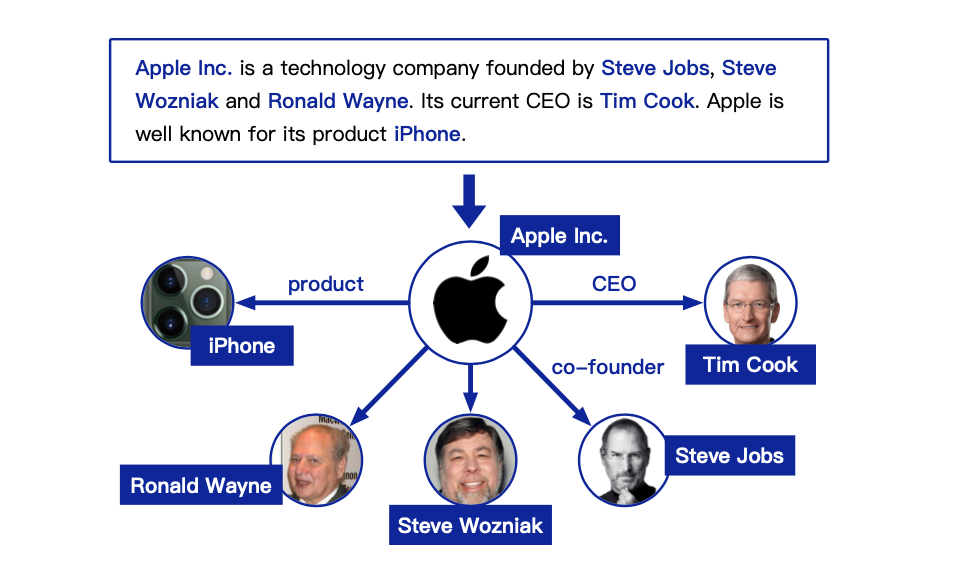
\includegraphics[width = 0.8\textwidth]{related_work/doc_re.png}
	\caption{一个文档级关系抽取的样例。给定一个包含有多个句子、多个实体的文档,模型需要抽取出文档中包含的所有关系事实。}
	\label{fig:related_work:doc_re}
\end{figure*}

目前大部分关系抽取的工作都是针对于句内关系的抽取,而忽略了文档级别句间关系的抽取。有许多关系事实往往涉及复杂的关系推理,用一句话难以表述清楚。在这样的情况下,句子级别关系抽取就无法有效地抽取出关系事实。据数据显示,在一篇文档中有$40.7\%$的关系事实必须通过多实体、跨句推理才能够抽取得到\cite{yao2019docred}。因此,将关系抽取任务从句子级别扩展到文档级别是非常必要的。

与句子级别关系抽取不同,一个文档中往往包含有非常多的实体,实体与实体之间也有着丰富多样的关系类型。同时,文档级别关系抽取任务的定义也与句子级别关系抽取定义有着一些不同。如图\ref{fig:related_work:doc_re}所示,文档级关系抽取旨在给定一篇文档及其中包含的实体时,抽取出这些实体之间所有的关系事实。在本小节,我将介绍主要文档级别关系抽取的数据集和现有的一些工作。

\subsection{文档级别关系抽取数据集}
从事文档级关系抽取的研究便要求有大规模的文档级别关系抽取的数据集,用来进行模型的训练及测试。随着文档级关系抽取受到越来越多的关注,也有学者相继提出了一些文档级别关系抽取的数据集。
Quirk et al.\cite{quirk2017distant}从PubMed\footnote{http://www.ncbi.nlm.nih.gov/pmc/}上获取了大量的无标注的生物医学文献,并将文档中的药物及基因实体识别出来,并与基因药物知识库(Gene Drug Knowledge Database,GDKD)中实体对齐,将在三句之内的关系,利用远程监督机制标注出来。Peng et al.\cite{peng2017cross}与前者类似,利用同样的机制从大量的无标注的生物医学文献中标注关系,但该工作主要关注于基因、药物、突变三者的多元关系。前面两个数据集关注到跨句关系推理,但都将数据语料限制在三句之内,无法真正做到文档级别关系抽取。并且这两个数据集没有进行人工标注,而使用带有噪音的远程监督数据来测试模型,这也导致了测试结果相对来说具有比较大的不可靠性。Li et al.\cite{li2016biocreative}提出了一个包含有$1,500$篇PubMed文档的手工标注数据集,该数据集专注于生物医学领域的“化学性疾病”这一关系。Yao et al.\cite{yao2019docred}提出DocRED数据集,该数据集基于维基百科进行构建,人工标注 $5,053$ 篇文档中包含的实体和关系。各个数据集具体的数据对比见\ref{table:related_work:dataset_stat}。

\begin{table}[]
\centering
\begin{tabular}{lrrrrrrr}
\toprule
Dataset             & \# Doc. & \# Word & \# Sent. & \# Ent.   & \# Rel. & \# Inst.  & \# Fact \\
\midrule
SemEval-2010 & -       & 205k    & 10,717   & 21,434    & 9       & 8,853     & 8,383   \\
ACE 2003-2004       & -       & 297k    & 12,783   & 46,108    & 24      & 16,771    & 16,536  \\
TACRED              & -       & 1,823k  & 53,791   & 152,527   & 41      & 21,773    & 5,976   \\
FewRel              & -       & 1,397k  & 56,109   & 72,124    & 100     & 70,000    & 55,803  \\
\midrule
BC5CDR              & 1,500,  & 282k    & 11,089   & 29,271    & 1       & 3,116     & 2,434   \\
DocRED\_a   & 50,053  & 1,002k  & 40,276   & 132,375   & 96      & 63,427    & 56,354  \\
DocRED\_d      & 101,873 & 21,368k & 828,115  & 2,558,350 & 96      & 1,508,320 & 881,298 \\
\bottomrule
\end{tabular}
\caption{各个关系抽取数据集的详细数据展示。其中Doc指文档数,Word指总共单词数量,Sent指句子数量,Ent指实体数量,Rel指关系数量,Inst指关系实例数量,Fact指关系事实数量。DocRED\_a指DocRED中人工标注数据集,DocRED\_d指DocRED中远程监督数据集。}
\label{table:related_work:dataset_stat}
\end{table}


\subsection{跨句关系抽取}
早期有很多工作关注于从跨句的关系抽取。许多学者\cite{swampillai2011extracting,yoshikawa2011coreference,quirk2017distant}聚焦于抽取出多个句子中的句法特征,利用句法特征将不同的句子连接在一起,再利用统计学习算法将特征分类到不同的关系中。常用的句法特征包括:实体指代特征、最短路径树、语法依存关系等。也有许多学者\cite{zeng2017incorporating,christopoulou2018walk}将不同的句子中的实体按照句内关系构成一个图,通过头尾实体之间的多跳路径来推理出实体之间的关系。\citet{peng2017cross,song2018n}则利用图神经网络(Graph Neural Network,GNN)来进行多实体、跨句的推理,图神经网络的运用给模型记忆能力、推理能力都带来了较大的提升。


\subsection{文档级关系抽取}
文档级关系抽取比之前工作提到的跨句关系抽取更加复杂,文档中多个句子具有较强的关联,且实体数量也要多很多。\citet{nguyen2018convolutional,li2018chemical}关注于生物医学、化学等特定领域的文档级关系抽取,并将之前句子级别关系抽取的模型直接利用至文档级别。但是由于传统模型,例如CNN、RNN等,在处理长的文本序列时,将遇到灾难性遗忘问题,因此模型无法充分利用实体的上下文信息。因此,有许多学者关注到使用图结构对篇章级别的文本进行建模,旨在建立起文档中长距离的、跨句子的信息流动,从而更好的实现多实体间的多步推理。\citet{quirk2017distant}构造了句内的依存边和句间的依存边来连接不同的实体。\citet{sahu2019inter}将词语作为结点,提出了五种边的类型:句法依存关系边、指代边、相邻句子边、相邻词语边、自环边,构造了一个文档级别的图结构,并利用图卷积神经网络(Graph Convolutional Neural Network)来学习结点表示,并将结点表示直接运用到最后关系分类中。而与此相反,\citet{christopoulou2019connecting}按照类似的方式构建了文档级的图结构,但其关注于边的表示的学习,并提出了一种以边为核心的图神经网络,将边的表示作为关系表示,运用于关系分类器中。

与之前的工作不同,本文提出的模型注重于通过预训练的模式高效地利用噪音很大的远程文档级监督数据。据我所知,本文是第一个在文档级别关系抽取中使用预训练的方式利用远程监督数据的工作。



\section{预训练模型}
\subsection{预训练语言模型}
预训练作为迁移学习的经典范式之一,在自然语言处理领域、计算机视觉领域都被广泛应用。计算机视觉领域许多研究也相继证明了基于预训练模型的迁移学习是十分有效的\cite{deng2009imagenet,yosinski2014transferable}。同样,在自然语言处理领域,预训练语言模型也得到了广泛的研究和应用。这些工作可以分成基于特征的预训练语言模型和基于微调的预训练语言模型两类。基于特征的预训练语言模型的工作\cite{mikolov2013distributed,pennington2014glove,peters2018deep}注重于将每一个词语映射到一个低维度、稠密的向量空间中,并将词语向量作为特征运用到下游的自然语言处理的相关任务当中。这些通过预训练得到的单词表示包含了丰富的句法特征和词意特征,所以这些向量经常被当做各种模型的输入,相比于利用随机初始化的词向量作为输入,这种方法在效果上取得了很大的提升。与基于特征的预训练语言模型仅运用预训练过程得到的词向量作为输入特征不同,基于微调的预训练语言模型将模型结构、参数都保留,作为下游任务模型训练的起点\cite{dai2015semi,howard2018universal,merity2017regularizing,devlin2019bert}。
其中\citet{devlin2019bert}提出的双向深度Transformer模型(Bert)取得了多个自然语言处理任务的最佳效果,因此该模型被广泛应用。本文的工作也是基于Bert模型开展实验。

\subsection{预训练关系表示学习}
随着预训练语言模型在很多任务上被证明是非常有效的,有许多学者\cite{du2018multi,wu2019enriching}也探索了如何将预训练语言模型运用到关系抽取任务上,这也在很多数据集上实现了最佳效果。也有许多学者聚焦于如何让模型学习可迁移的关系表示。\citet{wu2019open}提出了关系孪生网络,在有监督的数据集上让相同的关系有相似的表示,并将模型迁移至无监督数据上,实现了关系知识的迁移。进一步地,\citet{soares2019matching}提出,在大规模远程监督的句子级别关系抽取数据集上,学习有效的关系表示。与之前工作类似,该文章通过让出现在不同句子的相同的关系事实表示相近,让不同的关系事实表示距离变远来训练一个关系表示编码器。实验证明,该模型在关系抽取的有监督场景和少样本学习场景中效果均有明显提升。

然而,在文档级别远程监督数据中,噪音比例要远大于句子级别远程监督数据。因此,上述训练过程会因噪音过多而无法收敛。本文聚焦于在文档级别远程监督数据上进行模型预训练,通过提出的三种预训练任务充分学习关系表示。










% !TeX root = ../main.tex

\chapter{图表公式例子}
\label{cha:chapter02}

\section{其它例子}
\label{sec:other}

在第~\ref{cha:intro} 章中我们学习了贝叶斯公式~(\ref{equ:chap1:bayes}),这里我们复
习一下:
\begin{equation}
\label{equ:chap2:bayes}
p(y|\vx) = \frac{p(\vx,y)}{p(\vx)}=
\frac{p(\vx|y)p(y)}{p(\vx)}
\end{equation}

\subsection{绘图}
\label{sec:draw}

本模板不再预先装载任何绘图包(如 \pkg{pstricks,pgf} 等),完全由用户来决定。
个人觉得 \pkg{pgf} 不错,不依赖于 Postscript。此外还有很多针对 \LaTeX{} 的
 GUI 作图工具,如 XFig(jFig), WinFig, Tpx, Ipe, Dia, Inkscape, LaTeXPiX,
jPicEdt, jaxdraw 等等。

\subsection{插图}
\label{sec:graphs}

强烈推荐《\LaTeXe{} 插图指南》!关于子图形的使用细节请参看 \pkg{subcaption} 宏包的说明文档。

\subsubsection{一个图形}
\label{sec:onefig}
一般图形都是处在浮动环境中。之所以称为浮动是指最终排版效果图形的位置不一定与源文
件中的位置对应\footnote{This is not a bug, but a feature of \LaTeX!},这也是刚使
用 \LaTeX{} 同学可能遇到的问题。如果要强制固定浮动图形的位置,请使用 \pkg{float} 宏包,
它提供了 \texttt{[H]} 参数,比如图~\ref{fig:xfig1}。
\begin{figure}[H] % use float package if you want it here
  \centering
  
\includegraphics{thu-whole-logo.pdf}
  \caption{利用 Xfig 制图}
  \label{fig:xfig1}
\end{figure}

大学之道,在明明德,在亲民,在止于至善。知止而后有定;定而后能静;静而后能安;安
而后能虑;虑而后能得。物有本末,事有终始。知所先后,则近道矣。古之欲明明德于天
下者,先治其国;欲治其国者,先齐其家;欲齐其家者,先修其身;欲修其身者,先正其心;
欲正其心者,先诚其意;欲诚其意者,先致其知;致知在格物。物格而后知至;知至而后
意诚;意诚而后心正;心正而后身 修;身修而后家齐;家齐而后国治;国治而后天下
平。自天子以至于庶人,壹是皆以修身为本。其本乱而未治者 否矣。其所厚者薄,而其所
薄者厚,未之有也!

\hfill —— 《大学》


\subsubsection{多个图形}
\label{sec:multifig}

如果多个图形相互独立,并不共用一个图形计数器,那么
用 \texttt{minipage} 或者\texttt{parbox} 就可以。否则,请参看
图~\ref{fig:big1-subcaptionbox},它包含两个小图,分别是图~\ref{fig:subfig1}和
图~\ref{fig:subfig2}。推荐使用 \cs{subcaptionbox},因为可以像
图~\ref{fig:big1-subcaptionbox} 那样对齐子图的标题,也可以使用 \pkg{subcaption}
宏包的 \cs{subcaption}(放在 minipage中,用法同\cs{caption})或
是 \pkg{subfigure} 、\pkg{subtable}环境,像图~\ref{fig:big1-subfigure},不要再
用 \cs{subfloat}、\cs{subfigure} 和 \cs{subtable}。

\begin{figure}[h]
  \centering%
  \subcaptionbox{第一个小图形\label{fig:subfig1}}[3cm] %标题的长度,超过则会换行,如下一个小图。
    {
\includegraphics[height=3cm]{thu-fig-logo.pdf}}%
  \hspace{4em}%
  \subcaptionbox{第二个小图形,注意这个图略矮些。如果标题很长的话,它会自动换行\label{fig:subfig2}}
      {
\includegraphics[height=2cm]{thu-text-logo.pdf}}
  \caption{包含子图形的大图形(subcaptionbox示例)}
  \label{fig:big1-subcaptionbox}
\end{figure}
\begin{figure}[h]
  \centering%
  \begin{subfigure}{3cm}
    
\includegraphics[height=3cm]{thu-fig-logo.pdf}
    \caption{第一个小图形}
  \end{subfigure}%
  \hspace{4em}%
  \begin{subfigure}{0.5\textwidth}
    
\includegraphics[height=2cm]{thu-text-logo.pdf}
    \caption{第二个小图形,注意这个图略矮些。subfigure中同一行的子图在顶端对齐。}
  \end{subfigure}
  \caption{包含子图形的大图形(subfigure示例)}
  \label{fig:big1-subfigure}
\end{figure}

古之学者必有师。师者,所以传道受业解惑也。人非生而知之者,孰能无惑?惑而不从师,
其为惑也,终不解矣。生乎吾前,其闻道也固先乎吾,吾从而师之;生乎吾後,其闻道也亦
先乎吾,吾从而师之。吾师道也,夫庸知其年之先後生於吾乎!是故无贵无贱无长无少,道
之所存,师之所存也。

嗟乎!师道之不传也久矣,欲人之无惑也难矣。古之圣人,其出人也远矣,犹且从师而问焉;
今之众人,其下圣人也亦远矣,而耻学於师。是故圣益圣,愚益愚。圣人之所以为圣,愚
人之所以为愚,其皆出於此乎?爱其子,择师而教之,於其身也,则耻师焉,惑焉。彼童子
之师,授之书而习其句读者,非吾所谓传其道、解其惑者也。句读之不知,惑之不解,或师
焉,或不焉,小学而大遗,吾未见其明也。巫医、乐师、百工之人不耻相师,  士大夫之族
曰“师”曰“弟子”之云者,则群聚而笑之。问之,则曰:彼与彼年相若也,道相似也,位
卑则足羞,官盛则近谀。呜呼!师道之不复,可知矣。巫医、乐师、百工之人。吾子不齿,
今其智乃反不能及,其可怪也欤!圣人无常师。孔子师郯子、苌子、师襄、老聃。郯子之徒,
其贤不及孔子。孔子曰:“三人行,必有我师。”是故弟子不必不如师,师不必贤於弟子。
闻道有先後,术业有专攻,如是而已。

如果要把编号的两个图形并排,那么小页就非常有用了:
\begin{figure}
\begin{minipage}{0.48\textwidth}
  \centering
  
\includegraphics[height=2cm]{thu-whole-logo.pdf}
  \caption{并排第一个图}
  \label{fig:parallel1}
\end{minipage}\hfill
\begin{minipage}{0.48\textwidth}
  \centering
  
\includegraphics[height=2cm]{thu-whole-logo.pdf}
  \caption{并排第二个图}
  \label{fig:parallel2}
\end{minipage}
\end{figure}

李氏子蟠,年十七,好古文、六艺,经传皆通习之,不拘於时,学於余。余嘉其能行古
道,作师说以贻之。

\hfill —— 韩愈(唐)

% !TeX root = ../main.tex

\chapter{实验}
\label{cha:experiment}

本章节主要介绍模型实现的具体细节以及实验结果。本文在大规模的文档级关系抽取数据集上进行了测试,并针对于模型的各个预训练任务进行了消融实验,分析模型效果提升的关键因素。

\section{数据集及评价指标}

\begin{table}[]
\centering
\begin{tabular}{lcccc}
\toprule
类型             & \# Doc. & \# Rel & \# Inst. & \# Fact    \\
\midrule
训练集 			& 3,035   & 96     & 38,269   & 34,715     \\
验证集           & 1,000   & 96     & 12,332   & 11,790     \\
测试集           & 1,000   & 96     & 12,842   & 12,101     \\
远程监督集        & 101,873  & 96     &1,508,320 & 881,298    \\
\bottomrule
\end{tabular}
\caption{数据集的划分}
\label{table:experiment:docred_stat}
\end{table}

正如章节~\ref{cha:related_work}中所介绍,有许多学者相继提出了许多文档级别关系抽取的数据集。Quirk et al.\cite{quirk2017distant}和 Peng et al.\cite{peng2017cross}从PubMed上获取了大量的无标注的生物医学文献,并利用远程监督的机制对文献进行关系标注。这两个数据集关注于生物医学领域的关系知识,并且为了避免文档级别远程监督带来过多的错误标注样例,它们将文本限定在三个句子以内,且测试集也为远程监督数据,不利于模型的测试。Li et al.提出了一个包含有 $1,500$ 篇文档的手工标注的文档级别关系抽取数据集,但是该数据集只包含一种关系类型,无法体现模型的普适性。

因此,本文选择在数据集DocRED上验证模型的效果。DocRED是目前人工标注的最大的文档级关系抽取数据集。该数据集收集了大量来自于Wikipedia的文档,并利用命名实体识别工具将所有文档中的命名实体抽取出来,并将这些实体与Wikidata中的实体进行对齐,接着利用Wikidata中的关系事实标注出了大规模的文档级远程监督数据集。接着,从远程监督数据集中挑选出部分文档进行手工标注,分步标注出了命名实体、实体类别及实体之间的关系。DocRED中包含的文档在主题上具有很高的覆盖率。同时,实体类型也包含了人物、地点、组织、时间、数字五种常见类型以及其他。关系类型涵盖面也非常广,包含有科学、艺术、人物生活等方面的 $96$ 种类型。经过分析,该数据集要求模型具有模式识别、逻辑推理、指代消解和常识推理等能力。因此,该数据集能够很好地评测本文提出的模型的效果。在本文中,我使用远程监督集合进行模型预训练,利用手工标注数据进行模型的微调和测试。

在本节中,我使用了 $F_1$ 和 $IgnF_1$ 作为评价指标。其中 $IgnF_1$ 在\citet{yao2019docred}中定义。因为训练集与验证集和测试集包含的关系事实之间具有交集,为了避免模型通过记忆实体对的名称来进行关系的预测,便提出了 $IgnF_1$ 这个指标。该指标衡量的是在将验证集和测试集中包含的训练集中有的关系事实删除之后,模型的效果,该指标更能够反映出模型理解文本、理解关系的能力。


\section{基线模型}
本文挑选了以下基线模型与本文的模型进行对比。
\begin{itemize}
	\item \textbf{CNN/LSTM/BiLSTM}。这一类模型代表的是传统的序列模型,即将文档当做句子的扩展进行处理。这一类模型将词向量、位置向量、实体指代向量、实体类型向量、距离向量作为特征,并将这些特征全部拼接在一起,作为模型编码器的输入。之后这类模型将输入编码成一个隐向量序列。文档中每个实体提及的用该提及对应单词的隐向量的平均值来表示,而每个实体由该实体对应的提及的向量的平均来表示。最后,对于每一个实体对,用一个双线性层进行编码,得到该实体对对应的关系概率。
	\item \textbf{ContextAware}。与上述模型不同,该模型考虑一篇文章中具有多个实体对的情况,每个实体对的表示应该与其上下文的实体对表示有关。该模型利用双向长短时记忆网络编码文档,并同样利用双线性层获取每个实体对的表示。紧接着,模型利用注意力机制,将目标实体对作为询问值,将上下文中包含的其他实体对作为键值,计算权重。目标实体对的最终表示为上下文实体表示的加权平均。该模型考虑了多实体推理的情况,但是在文档级别关系抽取中,大量实体对是没有关系的,因此在加权平均时会引入较多噪音,所以在本文场景下,该模型并没有太多优势。
	\item \textbf{BERT}。预训练语言模型在自然语言处理领域的许多任务上都取得了很大的成功。因此,本文也采用BERT作为基线模型之一,与主模型进行对比。与章节~\ref{cha:model}中介绍的相同,该模型使用了实体标签来在模型中引入指代信息。文章中每一个实体提及的表示为该实体提及对应的实体开始标签的隐向量,并利用最大池化层来获取实体表示,最后利用双线性层获得关系表示。
	\item \textbf{BERT-Two-Step}。该模型基于BERT进行改造。该模型提出大量的负样例造成了标签极度不均的问题,该问题将导致模型训练出现偏差。因此,该模型提出利用两步策略进行预测。在获得了关系表示之后,首先判断该实体对之间是否有关系,若有关系,则在第二步中预测具体的关系种类。但是该模型并没有能够很好解决标签不均衡问题,因此它将标签不均衡问题集中在第一步的判断上,而导致第一步判断准确率并不是很高,因此相比于BERT模型,该模型并没有明显提升。
	\item \textbf{HIN-BERT}。该模型认为,文档级关系表示涉及非常复杂的推理过程,而推理应该在实体级、句子级、文档级三个级别依次进行。因此,该模型提出使用层次化的门控循环神经网络依次对实体、句子、文档进行编码,并在三个级别分别使用推理层进行信息融合。最后,模型通过结合三个层次的输出来预测实体对最终的关系。
\end{itemize}

这些模型都是在手工标注数据集上进行训练的,没有用到远程监督数据集中的信息。因此,为了充分对比基线模型与本文提出的主模型,本节将不仅给出上述模型在手工标注数据集上训练得到的结果,也将给出在远程监督数据集上训练得到的结果。从而,全面地验证本文提出的主模型的有效性。


\section{模型实现细节}

\smallskip
\noindent
\textbf{预训练参数设置。} 本文提出的模型基于BERT-base进行预训练。在预训练时,学习率设置为 $3 \times 10^{-5}$,在精度 FP16 下进行预训练。预训练时,batch size设置为 $16$。经过双线性层得到的关系的表示的维度设置为 $256$。对远程监督集合进行降噪时,本文保留了每一篇文章中得分最高的 $20$ 个实体对,其余实体对被认为是噪音丢弃了。并且对于预训练模型,我训练 $1000$ 个batch,即完成一个 epoch 的训练,总共训练了 9 个 epoch。

\smallskip
\noindent
\textbf{微调参数设置。} 在对模型进行微调时,学习率设置为 $1 \times 10^{-5}$,在精度 FP32 下进行微调。同时,微调时, batch size设置为 $4$。在对手工标注数据进行降噪时,为了让降噪后保留足够多的正样例,同时筛除足够多的负样例,本文保留了每一篇文章中得分最高的 $2 \times N_{\text{ent}}$,其中 $N_{\text{ent}}$ 是该文章中包含的实体数量。本文认为,实体数量越多则文章中包含的关系事实越多。微调时,所有结果均是在训练了不超过 $30$ 个epoch得到的。

\section{实验结果}

\begin{table}
\centering
\begin{tabular}{lcccc}
\toprule
             & \multicolumn{2}{c}{Dev} & \multicolumn{2}{c}{Test} \\
Model        & $F_1$      & $IgnF_1$   & $F_1$      & $IgnF_1$      \\ \midrule
\multicolumn{5}{c}{有监督场景} \\ \midrule
CNN*          & 43.45      & 41.58      & 42.26      & 40.33       \\
LSTM*         & 48.44      & 50.68      & 47.71      & 50.07       \\
BiLSTM*       & 50.94      & 48.87      & 51.06      & 48.78       \\
ContextAware* & 51.09      & 48.94      & 50.70      & 48.40       \\
BERT          & 55.67      & 53.32      & 56.17      & 53.66          \\
BERT-Two-Step $\clubsuit$ & 54.42      & --         & 53.92      & --          \\
HIN-BERT $\spadesuit$      & 56.31      & 54.29      & 55.60      & 53.70       \\
\midrule
\multicolumn{5}{c}{远程监督场景} \\ \midrule
CNN*          & 42.76      & 33.24      & 42.00      & 32.33       \\
LSTM*         & 49.92      & 39.37      & 48.88      & 38.27       \\
BiLSTM*       & 51.72      & 41.44      & 49.80      & 39.15       \\
ContextAware* & 51.39      & 40.47      & 50.12      & 39.16       \\
\midrule
BERT+D        & 57.42      & 55.88      & 57.20      & 55.53       \\
BERT+D+P    & \textbf{58.65}  & \textbf{57.00}  & \textbf{58.43}  & \textbf{56.68} \\ 
%Best in LeadBoard   & --      & --     & 62.30      & 60.10       \\ 
\bottomrule
\end{tabular}
\caption{主要的实验结果。其中标有*,$\clubsuit$ 和 $\spadesuit$ 的实验结果,分别是从 \citet{yao2019docred},\citet{wang2019fine}和\citet{tang2020hin}中获取的。其中基线模型给了有监督场景和远程监督场景两种结果。}
\label{main_result}
\end{table}

本文主要的实验结果如表格~\ref{main_result}中所示。其中 $D$ 表示降噪模块,$P$ 表示预训练。表格中分别给出了只进行降噪不预训练的模型效果,和既进行降噪又进行预训练的效果。观察表格中实验结果,我们可以得出以下结论:
\begin{itemize}
	\item 本文提出的模型显著优于所有的基线模型。在测试集中,相比于目前最好的基线模型HIN-BERT,本文提出的模型在 $F_1$ 和 $IgnF_1$ 两个指标上分别提升了 $2.83$ 和 $2.98$个点。这说明本文提出的降噪模块及三个预训练任务能够充分利用大规模远程监督数据上的信息,关于具体每一个预训练任务起到了多大的作用,将在之后的消融实验中进行讲述。
	\item 即使是不进行预训练的模型的结果(Bert+D)也能够超过最好的基线模型。这说明在文档级关系抽取中,太多的NA数据,确实给模型训练以及预测带来了较大的困难。这也说明了本文提出的降噪机制可以使模型效果有一个很明显的提升。该机制与具体模型无关,可以运用到各种各样的模型当中去。相比于对于NA数据有特殊处理的BERT-Two-Step模型,本文提出的降噪机制提升非常明显,进一步证明了模型降噪机制的有效。
	\item 在远程监督场景下训练的模型与在有监督场景下训练的相同模型相比,远程监督场景下训练的模型的效果相对来说都要差一些。这与句子级别远程监督实验不符。这说明在文档级别关系抽取中,远程监督机制引入了更多数据的同时,带来了远比句子级别要多的错误标注样例。这样的错误标注给模型训练带来了很大的偏差,从而使得模型效果下降。
	\item 本文提出的模型通过预训练的模式来利用远程监督数据。相比于远程监督场景下的基线模型,本文提出的模型效果是能够提升的。说明本文提出的三个预训练任务是十分有效的,能够在滤除噪音的同时,充分捕捉海量数据中的信息。
	\item 本文实现的基线模型BERT效果优于BERT-Two-Step模型,同时与HIN-BERT模型也能够达到类似的效果。这说明在BERT模型中引入实体标记,确实可以给模型带来指代信息,帮助模型更好地构建实体的表示,从而得到更具信息量的关系表示。
\end{itemize}

主实验的结果充分证明了本文提出模型的有效性,接下来为了分析各个预训练任务给模型带来的增益,本文继续开展了消融实验。


\section{消融实验}

\begin{table}
\centering
\begin{tabular}{lcccc}
\toprule
             & \multicolumn{2}{c}{Dev} & \multicolumn{2}{c}{Test} \\
模型        & $F_1$      & $IgnF_1$   & $F_1$      & $IgnF_1$      \\ \midrule
our model   & 58.65  & \textbf{57.00}  & \textbf{58.43}  & \textbf{56.68} \\
\midrule
\quad w/o M    & 58.39      & 56.76      & 57.60      & 55.81            \\
\quad w/o S    & 58.48      & 56.73      & 58.13      & 56.30            \\
\quad w/o N    & 57.19      & 55.61      & 56.71      & 54.94            \\ 
\midrule
\quad w/o Inter & \textbf{58.68}  & 56.96      & 57.72      & 55.87             \\
\quad w/o Intra & 57.78      & 56.18      & 57.62      & 55.89              \\
\bottomrule
\end{tabular}
\caption{在DocRED数据集上消融实验的结果。}
\label{ablation_study}
\end{table}

本文开展了一系列的消融实验来验证不同预训练任务的有效性。消融实验的实验结果如表格~\ref{ablation_study}中所示。其中我们将预训练任务一个一个从模型上移除,并观察移除之后模型的效果。其中 \textbf{w/o M},\textbf{w/o S},\textbf{w/o N}分别指的是模型移除了实体匹配、关系事实对齐、关系检测的结果。从消融实验的结果中可以得出以下结论:
\begin{itemize}
	\item 每一个预训练任务对应模型效果都是有帮助的。因为,从实验结果可以看出,删除任何一个任务,模型效果都会下降。
	\item 任务关系检测对于模型效果影响最大。从实验结果可以看出,当移除了关系检测这个任务之后,模型效果有了一个比较大幅的下降。甚至于,没有了关系检测任务之后的模型效果比没有预训练的模型(BERT+D)效果还要差。该任务旨在帮助模型学会区分正样例和负样例,而剩余两个预训练任务实体匹配和关系事实对齐,不涉及对于负样例的建模。因此,在没有关系检测任务的情况下,模型会将负样例和正样例混在一起,从而导致了效果的下降。
	\item 任务关系事实对齐对于模型效果影响最小。这说明其实区分不同的关系对于模型来说并不特别困难。
\end{itemize}

 \hspace*{\fill}
 
不仅如此,本文提出的实体匹配和关系对齐两个任务都包含跨文档和文档内两个部分的子任务,而关系事实对齐只包含跨文档任务。因此,为了探索跨文档和文档内两类子任务对于模型效果的影响,本文进一步开展了消融实验。其中 \textbf{w/o Inter} 是指移除了跨文档子任务后模型的效果,\textbf{w/o Intra} 是指移除了文档内子任务后模型的效果。从实验结果中,可以得出以下结论:
\begin{itemize}
	\item 删除了跨文档子任务之后,模型在验证集上的效果并没有明显的下降,甚至在 $F_1$ 指标上略高于主模型,但是在测试集上,模型效果就相对来说要差很多。这说明,没有了跨文档子任务之后,模型效果并不鲁棒,对于不同的测试集合来说,效果无法做到比较稳定,有比较大的起伏。
	\item 文档内子任务的删除对于模型效果有较大影响,因为一篇文档中会有多个实体、多个关系事实,模型在编码时需要同时考虑这些内容才能够获得更好的表示。当去除了文档内子任务时,模型将不会同时优化多个关系事实的表示,而是只尽量优化被挑选出的关系事实的表示。因此,模型效果出现下降。
\end{itemize}


\hspace*{\fill}
 
本节中,我使用了DocRED数据集来验证模型的有效性,模型利用DocRED的远程监督数据进行预训练,利用DocRED手工标注数据进行微调及测试。本文使用了 $F_1$ 和 $IgnF_1$ 作为评价指标。主实验表明,本文提出的模型可以超过所有基线模型,实现一个较好的效果。同时,本文还进行了消融实验验证了三个不同预训练任务的有效性,其中关系检测任务对于模型效果影响最大。紧接着,本文还对跨文档子任务和文档内子任务对模型效果的影响进行了研究。跨文档子任务可以帮助模型提升在不同测试集上的鲁棒性,文档内子任务可以帮助模型同时建模一篇文档内的多个关系事实。











% !TeX root = ../main.tex

\chapter{结论与未来工作}
\label{cha:conclusion}

本文提出了一种面向文档级别关系抽取的预训练机制。具体而言,本文提出了三种预训练任务:实体匹配、关系事实对齐、关系检测。这三个任务能够帮助模型在学习更加有效的实体表示、关系表示,并且能够辅助模型区分有关系实体对和无关系实体对。这在正负样例极度不均的文档级关系抽取中有着非常重要的作用。实验结果表明,与众多只利用了手工标注数据的基线模型相比,本文提出的预训练模型在文档级关系抽取任务上效果有了明显的提升。未来研究还有以下几个重要的方向:(1)利用更大规模的远程监督数据,本文只利用了DocRED数据集提供的十万份远程监督数据,在Wikipedia中有更大规模的数据可以使用;(2)更加普适的文档级预训练,本文目前只针对了文档级关系抽取这一任务进行测试,提出面向更多种多样的文档级任务将有很大的意义;(3)实现跨领域的文档级关系抽取,跨领域的关系抽取将帮助不同的领域快速构建知识图谱,能够很大推进多个领域的发展。这些方向将更好的帮助模型实现更有效、更多粒度的文档理解能力。

% 其它部分
\backmatter

%% 本科生要求的几个索引。
\listoffigures    % 插图索引
\listoftables     % 表格索引
\listofequations  % 公式索引

% 参考文献
%\bibliographystyle{thuthesis-numeric}      % 顺序编码制
% \bibliographystyle{thuthesis-author-year}  % 著者-出版年制
\bibliographystyle{thuthesis-bachelor}     % 本科生参考文献的著录格式
\bibliography{ref/refs}

% 致谢
% !TeX root = ../main.tex

\begin{acknowledgements}
  衷心感谢我的导师刘知远副教授。他在选题方向、实验设计、文章撰写上给我提供了细心全面的指导。不仅如此,通过他的言传身教,让我坚定了投身于自然语言处理研究的志向。他认真严谨的科研态度和扎实全面的学术素养都让我受益匪浅。
  
  我同样要感谢在我本科期间给予了我充分的支持与指导的实验室的师兄师姐们和同学们。涂存超、韩旭、谢若冰、姚远、钟皓曦几位学长帮助我入门自然语言处理领域,在我本科科研工作中,他们扮演了极其重要的角色,从完善想法、设计实验、文章撰写方面都给予了我大量的帮助,让我受益良多。张正彦、高天宇、王晓智三位师兄和同学在我困惑时伸出援助之手,与我讨论、为我答疑解惑,感谢他们一直以来的帮助与奉献。郭志芃师兄、陈慧敏师姐一直以来在学习、生活等多个方面给予了充分的关怀,他们的鼓励与帮助也成为了我不断成长的动力。
  
  我还要感谢我的朋友们,与你们在一起的欢声笑语将成为一生难忘的记忆。
  
  最后我要感谢我的家人。我的父母肖运锋先生和钟小芳女士给予我无条件的关怀与支持,我的姐姐肖朝荣女士给予了我充分的帮助与鼓励,他们是我在外求学中最坚强的后盾。
  
  
\end{acknowledgements}


% 声明
\statement

% 附录
\appendix
% % !TeX root = ../main.tex

\begin{survey}
\label{cha:survey}

\title{Title of the Survey}
\maketitle

写出至少 5000 外文印刷字符的调研阅读报告或者书面翻译 1-2 篇(不少于 2 万外文印刷符)。

It is impossible to cover in a single chapter every concept of mathematical
programming.\cite{tex} This chapter introduces only the basic concepts and techniques of
mathematical programming such that readers gain an understanding of them
throughout the book\cite{abrahams99tex,salomon1995advanced}.


\section{Single-Objective Programming}
The general form of single-objective programming (SOP) is written
as follows,
\begin{equation*} % 如果附录中的公式不想让它出现在公式索引中,那就请
                             % 用 equation*
\left\{\begin{array}{l}
\max \,\,f(x)\\[0.1 cm]
\mbox{subject to:} \\ [0.1 cm]
\qquad g_j(x)\le 0,\quad j=1,2,\cdots,p
\end{array}\right.
\end{equation*}
which maximizes a real-valued function $f$ of
$x=(x_1,x_2,\cdots,x_n)$ subject to a set of constraints.

\newcommand\Real{\mathbf{R}}
\newtheorem{mpdef}{Definition}[chapter]
\begin{mpdef}
In SOP, we call $x$ a decision vector, and
$x_1,x_2,\cdots,x_n$ decision variables. The function
$f$ is called the objective function. The set
\begin{equation*}
S=\left\{x\in\Real^n\bigm|g_j(x)\le 0,\,j=1,2,\cdots,p\right\}
\end{equation*}
is called the feasible set. An element $x$ in $S$ is called a
feasible solution.
\end{mpdef}

\newtheorem{mpdefop}[mpdef]{Definition}
\begin{mpdefop}
A feasible solution $x^*$ is called the optimal
solution of SOP if and only if
\begin{equation}
f(x^*)\ge f(x)
\end{equation}
for any feasible solution $x$.
\end{mpdefop}

One of the outstanding contributions to mathematical programming was known as
the Kuhn-Tucker conditions\ref{eq:ktc}. In order to introduce them, let us give
some definitions. An inequality constraint $g_j(x)\le 0$ is said to be active at
a point $x^*$ if $g_j(x^*)=0$. A point $x^*$ satisfying $g_j(x^*)\le 0$ is said
to be regular if the gradient vectors $\nabla g_j(x)$ of all active constraints
are linearly independent.

Let $x^*$ be a regular point of the constraints of SOP and assume that all the
functions $f(x)$ and $g_j(x),j=1,2,\cdots,p$ are differentiable. If $x^*$ is a
local optimal solution, then there exist Lagrange multipliers
$\lambda_j,j=1,2,\cdots,p$ such that the following Kuhn-Tucker conditions hold,
\begin{equation}
\label{eq:ktc}
\left\{\begin{array}{l}
    \nabla f(x^*)-\sum\limits_{j=1}^p\lambda_j\nabla g_j(x^*)=0\\[0.3cm]
    \lambda_jg_j(x^*)=0,\quad j=1,2,\cdots,p\\[0.2cm]
    \lambda_j\ge 0,\quad j=1,2,\cdots,p.
\end{array}\right.
\end{equation}
If all the functions $f(x)$ and $g_j(x),j=1,2,\cdots,p$ are convex and
differentiable, and the point $x^*$ satisfies the Kuhn-Tucker conditions
(\ref{eq:ktc}), then it has been proved that the point $x^*$ is a global optimal
solution of SOP.

\subsection{Linear Programming}
\label{sec:lp}

If the functions $f(x),g_j(x),j=1,2,\cdots,p$ are all linear, then SOP is called
a {\em linear programming}.

The feasible set of linear is always convex. A point $x$ is called an extreme
point of convex set $S$ if $x\in S$ and $x$ cannot be expressed as a convex
combination of two points in $S$. It has been shown that the optimal solution to
linear programming corresponds to an extreme point of its feasible set provided
that the feasible set $S$ is bounded. This fact is the basis of the {\em simplex
  algorithm} which was developed by Dantzig as a very efficient method for
solving linear programming.
\begin{table}[ht]
\centering
  \centering
  \caption*{Table~1\hskip1em This is an example for manually numbered table, which
    would not appear in the list of tables}
  \label{tab:badtabular2}
  \begin{tabular}[c]{|m{1.5cm}|c|c|c|c|c|c|}\hline
    \multicolumn{2}{|c|}{Network Topology} & \# of nodes &
    \multicolumn{3}{c|}{\# of clients} & Server \\\hline
    GT-ITM & Waxman Transit-Stub & 600 &
    \multirow{2}{2em}{2\%}&
    \multirow{2}{2em}{10\%}&
    \multirow{2}{2em}{50\%}&
    \multirow{2}{1.2in}{Max. Connectivity}\\\cline{1-3}
    \multicolumn{2}{|c|}{Inet-2.1} & 6000 & & & &\\\hline
    \multirow{2}{1.5cm}{Xue} & Rui  & Ni &\multicolumn{4}{c|}{\multirow{2}*{\thuthesis}}\\\cline{2-3}
    & \multicolumn{2}{c|}{ABCDEF} &\multicolumn{4}{c|}{} \\\hline
\end{tabular}
\end{table}

Roughly speaking, the simplex algorithm examines only the extreme points of the
feasible set, rather than all feasible points. At first, the simplex algorithm
selects an extreme point as the initial point. The successive extreme point is
selected so as to improve the objective function value. The procedure is
repeated until no improvement in objective function value can be made. The last
extreme point is the optimal solution.

\subsection{Nonlinear Programming}

If at least one of the functions $f(x),g_j(x),j=1,2,\cdots,p$ is nonlinear, then
SOP is called a {\em nonlinear programming}.

A large number of classical optimization methods have been developed to treat
special-structural nonlinear programming based on the mathematical theory
concerned with analyzing the structure of problems.
\begin{figure}[h]
  \centering
  
\includegraphics{thu-lib-logo.pdf}
  \caption*{Figure~1\quad This is an example for manually numbered figure,
    which would not appear in the list of figures}
  \label{tab:badfigure2}
\end{figure}

Now we consider a nonlinear programming which is confronted solely with
maximizing a real-valued function with domain $\Real^n$.  Whether derivatives are
available or not, the usual strategy is first to select a point in $\Real^n$ which
is thought to be the most likely place where the maximum exists. If there is no
information available on which to base such a selection, a point is chosen at
random. From this first point an attempt is made to construct a sequence of
points, each of which yields an improved objective function value over its
predecessor. The next point to be added to the sequence is chosen by analyzing
the behavior of the function at the previous points. This construction continues
until some termination criterion is met. Methods based upon this strategy are
called {\em ascent methods}, which can be classified as {\em direct methods},
{\em gradient methods}, and {\em Hessian methods} according to the information
about the behavior of objective function $f$. Direct methods require only that
the function can be evaluated at each point. Gradient methods require the
evaluation of first derivatives of $f$. Hessian methods require the evaluation
of second derivatives. In fact, there is no superior method for all
problems. The efficiency of a method is very much dependent upon the objective
function.

\subsection{Integer Programming}

{\em Integer programming} is a special mathematical programming in which all of
the variables are assumed to be only integer values. When there are not only
integer variables but also conventional continuous variables, we call it {\em
  mixed integer programming}. If all the variables are assumed either 0 or 1,
then the problem is termed a {\em zero-one programming}. Although integer
programming can be solved by an {\em exhaustive enumeration} theoretically, it
is impractical to solve realistically sized integer programming problems. The
most successful algorithm so far found to solve integer programming is called
the {\em branch-and-bound enumeration} developed by Balas (1965) and Dakin
(1965). The other technique to integer programming is the {\em cutting plane
  method} developed by Gomory (1959).

\hfill\textit{Uncertain Programming\/}\quad(\textsl{BaoDing Liu, 2006.2})

\bibliographystyle{plainnat}
\bibliography{ref/refs,ref/appendix}

\end{survey}
       % 本科生:外文资料的调研阅读报告
% % !TeX root = ../main.tex

\begin{translation}
\label{cha:translation}

\title{书面翻译题目}
\maketitle

\section{单目标规划}
北冥有鱼,其名为鲲。鲲之大,不知其几千里也。化而为鸟,其名为鹏。鹏之背,不知其几
千里也。怒而飞,其翼若垂天之云。是鸟也,海运则将徙于南冥。南冥者,天池也。
\begin{equation}\tag*{(123)}
 p(y|\mathbf{x}) = \frac{p(\mathbf{x},y)}{p(\mathbf{x})}=
\frac{p(\mathbf{x}|y)p(y)}{p(\mathbf{x})}
\end{equation}

吾生也有涯,而知也无涯。以有涯随无涯,殆已!已而为知者,殆而已矣!为善无近名,为
恶无近刑,缘督以为经,可以保身,可以全生,可以养亲,可以尽年。

\subsection{线性规划}
庖丁为文惠君解牛,手之所触,肩之所倚,足之所履,膝之所倚,砉然响然,奏刀騞然,莫
不中音,合于桑林之舞,乃中经首之会。
\begin{table}[ht]
\centering
  \centering
  \caption*{表~1\hskip1em 这是手动编号但不出现在索引中的一个表格例子}
  \label{tab:badtabular3}
  \begin{tabular}[c]{|m{1.5cm}|c|c|c|c|c|c|}\hline
    \multicolumn{2}{|c|}{Network Topology} & \# of nodes &
    \multicolumn{3}{c|}{\# of clients} & Server \\\hline
    GT-ITM & Waxman Transit-Stub & 600 &
    \multirow{2}{2em}{2\%}&
    \multirow{2}{2em}{10\%}&
    \multirow{2}{2em}{50\%}&
    \multirow{2}{1.2in}{Max. Connectivity}\\\cline{1-3}
    \multicolumn{2}{|c|}{Inet-2.1} & 6000 & & & &\\\hline
    \multirow{2}{1.5cm}{Xue} & Rui  & Ni &\multicolumn{4}{c|}{\multirow{2}*{\thuthesis}}\\\cline{2-3}
    & \multicolumn{2}{c|}{ABCDEF} &\multicolumn{4}{c|}{} \\\hline
\end{tabular}
\end{table}

文惠君曰:“嘻,善哉!技盖至此乎?”庖丁释刀对曰:“臣之所好者道也,进乎技矣。始臣之
解牛之时,所见无非全牛者;三年之后,未尝见全牛也;方今之时,臣以神遇而不以目视,
官知止而神欲行。依乎天理,批大郤,导大窾,因其固然。技经肯綮之未尝,而况大坬乎!
良庖岁更刀,割也;族庖月更刀,折也;今臣之刀十九年矣,所解数千牛矣,而刀刃若新发
于硎。彼节者有间而刀刃者无厚,以无厚入有间,恢恢乎其于游刃必有余地矣。是以十九年
而刀刃若新发于硎。虽然,每至于族,吾见其难为,怵然为戒,视为止,行为迟,动刀甚微,
謋然已解,如土委地。提刀而立,为之而四顾,为之踌躇满志,善刀而藏之。”

文惠君曰:“善哉!吾闻庖丁之言,得养生焉。”


\subsection{非线性规划}
孔子与柳下季为友,柳下季之弟名曰盗跖。盗跖从卒九千人,横行天下,侵暴诸侯。穴室枢
户,驱人牛马,取人妇女。贪得忘亲,不顾父母兄弟,不祭先祖。所过之邑,大国守城,小
国入保,万民苦之。孔子谓柳下季曰:“夫为人父者,必能诏其子;为人兄者,必能教其弟。
若父不能诏其子,兄不能教其弟,则无贵父子兄弟之亲矣。今先生,世之才士也,弟为盗
跖,为天下害,而弗能教也,丘窃为先生羞之。丘请为先生往说之。”
\begin{figure}[h]
  \centering
  
\includegraphics{thu-whole-logo.pdf}
  \caption*{图~1\hskip1em 这是手动编号但不出现索引中的图片的例子}
  \label{tab:badfigure3}
\end{figure}

柳下季曰:“先生言为人父者必能诏其子,为人兄者必能教其弟,若子不听父之诏,弟不受
兄之教,虽今先生之辩,将奈之何哉?且跖之为人也,心如涌泉,意如飘风,强足以距敌,
辩足以饰非。顺其心则喜,逆其心则怒,易辱人以言。先生必无往。”

孔子不听,颜回为驭,子贡为右,往见盗跖。

\subsection{整数规划}
盗跖乃方休卒徒大山之阳,脍人肝而餔之。孔子下车而前,见谒者曰:“鲁人孔丘,闻将军
高义,敬再拜谒者。”谒者入通。盗跖闻之大怒,目如明星,发上指冠,曰:“此夫鲁国之
巧伪人孔丘非邪?为我告之:尔作言造语,妄称文、武,冠枝木之冠,带死牛之胁,多辞缪
说,不耕而食,不织而衣,摇唇鼓舌,擅生是非,以迷天下之主,使天下学士不反其本,妄
作孝弟,而侥幸于封侯富贵者也。子之罪大极重,疾走归!不然,我将以子肝益昼餔之膳。”


\nocite{abrahams99tex,salomon1995advanced}
\bibliographystyle{plainnat}
\bibliography{ref/appendix}

% 也可以使用 thebiliography 环境手写
% \begin{thebibliography}{2}
%   \bibitem{abrahams99tex}
%   P.~W. Abrahams, K.~Berry, and K.~A. Hargreaves, \emph{{\TeX} for the
%     Impatient}.\hskip 1em plus 0.5em minus 0.4em\relax Addison-Wesley, 1990.

%   \bibitem{salomon1995advanced}
%   D.~Salomon, ``The advanced {\TeX}book.''\hskip 1em plus 0.5em minus 0.4em\relax
%     New York: Springer, 1995.
% \end{thebibliography}


\end{translation}
  % 本科生:外文资料的书面翻译
\chapter{单目标规划}

As one of the most widely used techniques in operations
research, \emph{ mathematical programming} is defined as a means of maximizing a
quantity known as \emph{bjective function}, subject to a set of constraints
represented by equations and inequalities. Some known subtopics of mathematical
programming are linear programming, nonlinear programming, multiobjective
programming, goal programming, dynamic programming, and multilevel
programming.

It is impossible to cover in a single chapter every concept of mathematical
programming. This chapter introduces only the basic concepts and techniques of
mathematical programming such that readers gain an understanding of them
throughout the book.


\section{Single-Objective Programming}
The general form of single-objective programming (SOP) is written
as follows,
\begin{equation*} % 如果附录中的公式不想让它出现在公式索引中,那就请
                             % 用 equation*
\left\{\begin{array}{l}
\max \,\,f(x)\\[0.1 cm]
\mbox{subject to:} \\ [0.1 cm]
\qquad g_j(x)\le 0,\quad j=1,2,\cdots,p
\end{array}\right.
\end{equation*}
which maximizes a real-valued function $f$ of
$x=(x_1,x_2,\cdots,x_n)$ subject to a set of constraints.

\newcommand\Real{\mathbf{R}}
\newtheorem{mpdef}{Definition}[chapter]
\begin{mpdef}
In SOP, we call $x$ a decision vector, and
$x_1,x_2,\cdots,x_n$ decision variables. The function
$f$ is called the objective function. The set
\begin{equation*}
S=\left\{x\in\Real^n\bigm|g_j(x)\le 0,\,j=1,2,\cdots,p\right\}
\end{equation*}
is called the feasible set. An element $x$ in $S$ is called a
feasible solution.
\end{mpdef}

\newtheorem{mpdefop}[mpdef]{Definition}
\begin{mpdefop}
A feasible solution $x^*$ is called the optimal
solution of SOP if and only if
\begin{equation}
f(x^*)\ge f(x)
\end{equation}
for any feasible solution $x$.
\end{mpdefop}

One of the outstanding contributions to mathematical programming was known as
the Kuhn-Tucker conditions\ref{eq:ktc}. In order to introduce them, let us give
some definitions. An inequality constraint $g_j(x)\le 0$ is said to be active at
a point $x^*$ if $g_j(x^*)=0$. A point $x^*$ satisfying $g_j(x^*)\le 0$ is said
to be regular if the gradient vectors $\nabla g_j(x)$ of all active constraints
are linearly independent.

Let $x^*$ be a regular point of the constraints of SOP and assume that all the
functions $f(x)$ and $g_j(x),j=1,2,\cdots,p$ are differentiable. If $x^*$ is a
local optimal solution, then there exist Lagrange multipliers
$\lambda_j,j=1,2,\cdots,p$ such that the following Kuhn-Tucker conditions hold,
\begin{equation}
\label{eq:ktc}
\left\{\begin{array}{l}
    \nabla f(x^*)-\sum\limits_{j=1}^p\lambda_j\nabla g_j(x^*)=0\\[0.3cm]
    \lambda_jg_j(x^*)=0,\quad j=1,2,\cdots,p\\[0.2cm]
    \lambda_j\ge 0,\quad j=1,2,\cdots,p.
\end{array}\right.
\end{equation}
If all the functions $f(x)$ and $g_j(x),j=1,2,\cdots,p$ are convex and
differentiable, and the point $x^*$ satisfies the Kuhn-Tucker conditions
(\ref{eq:ktc}), then it has been proved that the point $x^*$ is a global optimal
solution of SOP.

\subsection{Linear Programming}
\label{sec:lp}

If the functions $f(x),g_j(x),j=1,2,\cdots,p$ are all linear, then SOP is called
a {\em linear programming}.

The feasible set of linear is always convex. A point $x$ is called an extreme
point of convex set $S$ if $x\in S$ and $x$ cannot be expressed as a convex
combination of two points in $S$. It has been shown that the optimal solution to
linear programming corresponds to an extreme point of its feasible set provided
that the feasible set $S$ is bounded. This fact is the basis of the {\em simplex
  algorithm} which was developed by Dantzig as a very efficient method for
solving linear programming.
\begin{table}[ht]
\centering
  \centering
  \caption*{Table~1\hskip1em This is an example for manually numbered table, which
    would not appear in the list of tables}
  \label{tab:badtabular2}
  \begin{tabular}[c]{|m{1.5cm}|c|c|c|c|c|c|}\hline
    \multicolumn{2}{|c|}{Network Topology} & \# of nodes &
    \multicolumn{3}{c|}{\# of clients} & Server \\\hline
    GT-ITM & Waxman Transit-Stub & 600 &
    \multirow{2}{2em}{2\%}&
    \multirow{2}{2em}{10\%}&
    \multirow{2}{2em}{50\%}&
    \multirow{2}{1.2in}{Max. Connectivity}\\\cline{1-3}
    \multicolumn{2}{|c|}{Inet-2.1} & 6000 & & & &\\\hline
    \multirow{2}{1.5cm}{Xue} & Rui  & Ni &\multicolumn{4}{c|}{\multirow{2}*{\thuthesis}}\\\cline{2-3}
    & \multicolumn{2}{c|}{ABCDEF} &\multicolumn{4}{c|}{} \\\hline
\end{tabular}
\end{table}

Roughly speaking, the simplex algorithm examines only the extreme points of the
feasible set, rather than all feasible points. At first, the simplex algorithm
selects an extreme point as the initial point. The successive extreme point is
selected so as to improve the objective function value. The procedure is
repeated until no improvement in objective function value can be made. The last
extreme point is the optimal solution.

\subsection{Nonlinear Programming}

If at least one of the functions $f(x),g_j(x),j=1,2,\cdots,p$ is nonlinear, then
SOP is called a {\em nonlinear programming}.

A large number of classical optimization methods have been developed to treat
special-structural nonlinear programming based on the mathematical theory
concerned with analyzing the structure of problems.
\begin{figure}[h]
  \centering
  
\includegraphics{thu-lib-logo.pdf}
  \caption*{Figure~1\quad This is an example for manually numbered figure,
    which would not appear in the list of figures}
  \label{tab:badfigure2}
\end{figure}

Now we consider a nonlinear programming which is confronted solely with
maximizing a real-valued function with domain $\Real^n$.  Whether derivatives are
available or not, the usual strategy is first to select a point in $\Real^n$ which
is thought to be the most likely place where the maximum exists. If there is no
information available on which to base such a selection, a point is chosen at
random. From this first point an attempt is made to construct a sequence of
points, each of which yields an improved objective function value over its
predecessor. The next point to be added to the sequence is chosen by analyzing
the behavior of the function at the previous points. This construction continues
until some termination criterion is met. Methods based upon this strategy are
called {\em ascent methods}, which can be classified as {\em direct methods},
{\em gradient methods}, and {\em Hessian methods} according to the information
about the behavior of objective function $f$. Direct methods require only that
the function can be evaluated at each point. Gradient methods require the
evaluation of first derivatives of $f$. Hessian methods require the evaluation
of second derivatives. In fact, there is no superior method for all
problems. The efficiency of a method is very much dependent upon the objective
function.

\subsection{Integer Programming}

{\em Integer programming} is a special mathematical programming in which all of
the variables are assumed to be only integer values. When there are not only
integer variables but also conventional continuous variables, we call it {\em
  mixed integer programming}. If all the variables are assumed either 0 or 1,
then the problem is termed a {\em zero-one programming}. Although integer
programming can be solved by an {\em exhaustive enumeration} theoretically, it
is impractical to solve realistically sized integer programming problems. The
most successful algorithm so far found to solve integer programming is called
the {\em branch-and-bound enumeration} developed by Balas (1965) and Dakin
(1965). The other technique to integer programming is the {\em cutting plane
  method} developed by Gomory (1959).

\hfill\textit{Uncertain Programming\/}\quad(\textsl{BaoDing Liu, 2006.2})

\section{单目标规划}
北冥有鱼,其名为鲲。鲲之大,不知其几千里也。化而为鸟,其名为鹏。鹏之背,不知其几
千里也。怒而飞,其翼若垂天之云。是鸟也,海运则将徙于南冥。南冥者,天池也。
\begin{equation}\tag*{(123)}
 p(y|\mathbf{x}) = \frac{p(\mathbf{x},y)}{p(\mathbf{x})}=
\frac{p(\mathbf{x}|y)p(y)}{p(\mathbf{x})}
\end{equation}

吾生也有涯,而知也无涯。以有涯随无涯,殆已!已而为知者,殆而已矣!为善无近名,为
恶无近刑,缘督以为经,可以保身,可以全生,可以养亲,可以尽年。

\subsection{线性规划}
庖丁为文惠君解牛,手之所触,肩之所倚,足之所履,膝之所倚,砉然响然,奏刀騞然,莫
不中音,合于桑林之舞,乃中经首之会。
\begin{table}[ht]
\centering
  \centering
  \caption*{表~1\hskip1em 这是手动编号但不出现在索引中的一个表格例子}
  \label{tab:badtabular3}
  \begin{tabular}[c]{|m{1.5cm}|c|c|c|c|c|c|}\hline
    \multicolumn{2}{|c|}{Network Topology} & \# of nodes &
    \multicolumn{3}{c|}{\# of clients} & Server \\\hline
    GT-ITM & Waxman Transit-Stub & 600 &
    \multirow{2}{2em}{2\%}&
    \multirow{2}{2em}{10\%}&
    \multirow{2}{2em}{50\%}&
    \multirow{2}{1.2in}{Max. Connectivity}\\\cline{1-3}
    \multicolumn{2}{|c|}{Inet-2.1} & 6000 & & & &\\\hline
    \multirow{2}{1.5cm}{Xue} & Rui  & Ni &\multicolumn{4}{c|}{\multirow{2}*{\thuthesis}}\\\cline{2-3}
    & \multicolumn{2}{c|}{ABCDEF} &\multicolumn{4}{c|}{} \\\hline
\end{tabular}
\end{table}

文惠君曰:“嘻,善哉!技盖至此乎?”庖丁释刀对曰:“臣之所好者道也,进乎技矣。始臣之
解牛之时,所见无非全牛者;三年之后,未尝见全牛也;方今之时,臣以神遇而不以目视,
官知止而神欲行。依乎天理,批大郤,导大窾,因其固然。技经肯綮之未尝,而况大坬乎!
良庖岁更刀,割也;族庖月更刀,折也;今臣之刀十九年矣,所解数千牛矣,而刀刃若新发
于硎。彼节者有间而刀刃者无厚,以无厚入有间,恢恢乎其于游刃必有余地矣。是以十九年
而刀刃若新发于硎。虽然,每至于族,吾见其难为,怵然为戒,视为止,行为迟,动刀甚微,
謋然已解,如土委地。提刀而立,为之而四顾,为之踌躇满志,善刀而藏之。”

文惠君曰:“善哉!吾闻庖丁之言,得养生焉。”


\subsection{非线性规划}
孔子与柳下季为友,柳下季之弟名曰盗跖。盗跖从卒九千人,横行天下,侵暴诸侯。穴室枢
户,驱人牛马,取人妇女。贪得忘亲,不顾父母兄弟,不祭先祖。所过之邑,大国守城,小
国入保,万民苦之。孔子谓柳下季曰:“夫为人父者,必能诏其子;为人兄者,必能教其弟。
若父不能诏其子,兄不能教其弟,则无贵父子兄弟之亲矣。今先生,世之才士也,弟为盗
跖,为天下害,而弗能教也,丘窃为先生羞之。丘请为先生往说之。”
\begin{figure}[h]
  \centering
  
\includegraphics{thu-whole-logo.pdf}
  \caption*{图~1\hskip1em 这是手动编号但不出现索引中的图片的例子}
  \label{tab:badfigure3}
\end{figure}

柳下季曰:“先生言为人父者必能诏其子,为人兄者必能教其弟,若子不听父之诏,弟不受
兄之教,虽今先生之辩,将奈之何哉?且跖之为人也,心如涌泉,意如飘风,强足以距敌,
辩足以饰非。顺其心则喜,逆其心则怒,易辱人以言。先生必无往。”

孔子不听,颜回为驭,子贡为右,往见盗跖。

\subsection{整数规划}
盗跖乃方休卒徒大山之阳,脍人肝而餔之。孔子下车而前,见谒者曰:“鲁人孔丘,闻将军
高义,敬再拜谒者。”谒者入通。盗跖闻之大怒,目如明星,发上指冠,曰:“此夫鲁国之
巧伪人孔丘非邪?为我告之:尔作言造语,妄称文、武,冠枝木之冠,带死牛之胁,多辞缪
说,不耕而食,不织而衣,摇唇鼓舌,擅生是非,以迷天下之主,使天下学士不反其本,妄
作孝弟,而侥幸于封侯富贵者也。子之罪大极重,疾走归!不然,我将以子肝益昼餔之膳。”


% 个人简历
% !TeX root = ../main.tex

\begin{resume}

  \resumeitem{个人简历}

  1998 年 8 月 9 日出生于 江西 省 兴国 县。

  2016 年 8 月考入 清华 大学 计算机科学与技术 系 计算机科学与技术 专业 攻读 学士 学位至今。

  \researchitem{发表的学术论文} % 发表的和录用的合在一起

  % 1. 已经刊载的学术论文(本人是第一作者,或者导师为第一作者本人是第二作者)
  \begin{publications}
    \item Yang Y, Ren T L, Zhang L T, et al. Miniature microphone with silicon-
      based ferroelectric thin films. Integrated Ferroelectrics, 2003,
      52:229-235. (SCI 收录, 检索号:758FZ.)
    \item 杨轶, 张宁欣, 任天令, 等. 硅基铁电微声学器件中薄膜残余应力的研究. 中国机
      械工程, 2005, 16(14):1289-1291. (EI 收录, 检索号:0534931 2907.)
    \item 杨轶, 张宁欣, 任天令, 等. 集成铁电器件中的关键工艺研究. 仪器仪表学报,
      2003, 24(S4):192-193. (EI 源刊.)
  \end{publications}

  % 2. 尚未刊载,但已经接到正式录用函的学术论文(本人为第一作者,或者
  %    导师为第一作者本人是第二作者)。
  \begin{publications}[before=\publicationskip,after=\publicationskip]
    \item Yang Y, Ren T L, Zhu Y P, et al. PMUTs for handwriting recognition. In
      press. (已被 Integrated Ferroelectrics 录用. SCI 源刊.)
  \end{publications}

  % 3. 其他学术论文。可列出除上述两种情况以外的其他学术论文,但必须是
  %    已经刊载或者收到正式录用函的论文。
  \begin{publications}
    \item Wu X M, Yang Y, Cai J, et al. Measurements of ferroelectric MEMS
      microphones. Integrated Ferroelectrics, 2005, 69:417-429. (SCI 收录, 检索号
      :896KM)
    \item 贾泽, 杨轶, 陈兢, 等. 用于压电和电容微麦克风的体硅腐蚀相关研究. 压电与声
      光, 2006, 28(1):117-119. (EI 收录, 检索号:06129773469)
    \item 伍晓明, 杨轶, 张宁欣, 等. 基于MEMS技术的集成铁电硅微麦克风. 中国集成电路,
      2003, 53:59-61.
  \end{publications}

  \researchitem{研究成果} % 有就写,没有就删除
  \begin{achievements}
    \item 任天令, 杨轶, 朱一平, 等. 硅基铁电微声学传感器畴极化区域控制和电极连接的
      方法: 中国, CN1602118A. (中国专利公开号)
    \item Ren T L, Yang Y, Zhu Y P, et al. Piezoelectric micro acoustic sensor
      based on ferroelectric materials: USA, No.11/215, 102. (美国发明专利申请号)
  \end{achievements}

\end{resume}


% 本科生的综合论文训练记录表
% 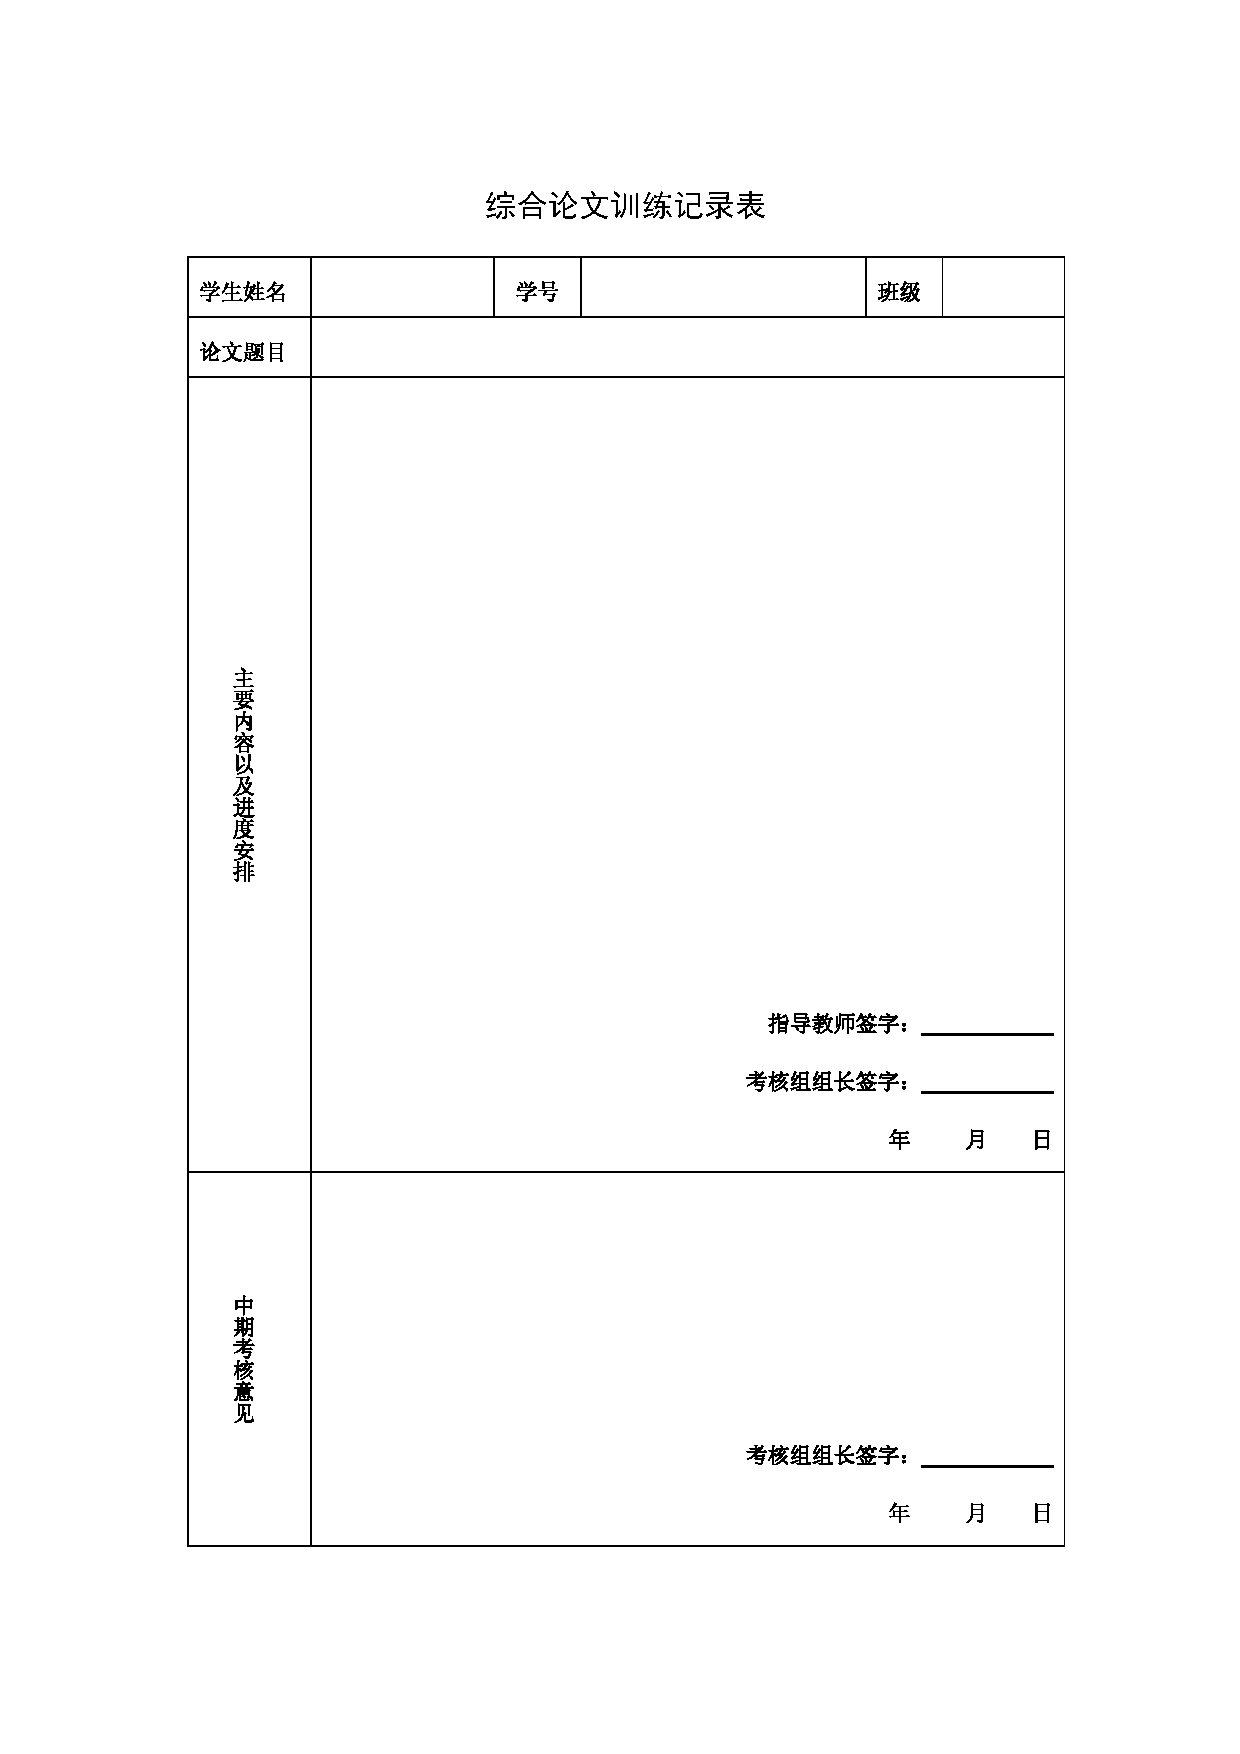
\includepdf[pages=-]{scan-record.pdf}

\end{document}
